\documentclass[degree=bachelor,tocarialchapter]{thuthesis}
% 选项
%   degree=[bachelor|master|doctor|postdoctor], % 必选,学位类型
%   language=[chinese|english], % 可选(默认:chinese),论文的主要语言
%   secret,                % 可选(默认:关闭),是否有密级
%   tocarialchapter,       % 可选(默认:关闭),章目录中使用黑体(这项表示同时打开下面两项)
%   tocarialchapterentry,  % 可选(默认:关闭),单独控制章标题在目录中使用黑体
%   tocarialchapterpage,   % 可选(默认:关闭),单独控制章页码在目录中使用黑体

% 所有其它可能用到的包都统一放到这里了,可以根据自己的实际添加或者删除。
\usepackage{thuthesis}

% 定义所有的图片文件在 figures 子目录下
\graphicspath{{figures/}}

% 可以在这里修改配置文件中的定义。导言区可以使用中文。
% \def\myname{薛瑞尼}

\begin{document}

%%% 封面部分
\frontmatter
\thusetup{
  %******************************
  % 注意:
  %   1. 配置里面不要出现空行
  %   2. 不需要的配置信息可以删除
  %******************************
  %
  %=====
  % 秘级
  %=====
  secretlevel={秘密},
  secretyear={10},
  %
  %=========
  % 中文信息
  %=========
  ctitle={面向稀疏矩阵的Allreduce\\优化技术研究},
  cdegree={工学硕士},
  cdepartment={计算机科学与技术系},
  cmajor={计算机科学与技术},
  cauthor={师天麾},
  csupervisor={翟季冬副教授},
  %cassosupervisor={陈文光教授}, % 副指导老师
  %ccosupervisor={某某某教授}, % 联合指导老师
  % 日期自动使用当前时间,若需指定按如下方式修改:
  % cdate={超新星纪元},
  %
  % 博士后专有部分
  catalognumber     = {分类号},  % 可以留空
  udc               = {UDC},  % 可以留空
  id                = {编号},  % 可以留空: id={},
  cfirstdiscipline  = {计算机科学与技术},  % 流动站(一级学科)名称
  cseconddiscipline = {系统结构},  % 专 业(二级学科)名称
  postdoctordate    = {2009 年 7 月——2011 年 7 月},  % 工作完成日期
  postdocstartdate  = {2009 年 7 月 1 日},  % 研究工作起始时间
  postdocenddate    = {2011 年 7 月 1 日},  % 研究工作期满时间
  %
  %=========
  % 英文信息
  %=========
  etitle={An Introduction to \LaTeX{} Thesis Template of Tsinghua University v\version},
  % 这块比较复杂,需要分情况讨论:
  % 1. 学术型硕士
  %    edegree:必须为Master of Arts或Master of Science(注意大小写)
  %             “哲学、文学、历史学、法学、教育学、艺术学门类,公共管理学科
  %              填写Master of Arts,其它填写Master of Science”
  %    emajor:“获得一级学科授权的学科填写一级学科名称,其它填写二级学科名称”
  % 2. 专业型硕士
  %    edegree:“填写专业学位英文名称全称”
  %    emajor:“工程硕士填写工程领域,其它专业学位不填写此项”
  % 3. 学术型博士
  %    edegree:Doctor of Philosophy(注意大小写)
  %    emajor:“获得一级学科授权的学科填写一级学科名称,其它填写二级学科名称”
  % 4. 专业型博士
  %    edegree:“填写专业学位英文名称全称”
  %    emajor:不填写此项
  edegree={Doctor of Engineering},
  emajor={Computer Science and Technology},
  eauthor={Xue Ruini},
  esupervisor={Professor Zheng Weimin},
  eassosupervisor={Chen Wenguang},
  % 日期自动生成,若需指定按如下方式修改:
  % edate={December, 2005}
  %
  % 关键词用“英文逗号”分割
  ckeywords={Allreduce, 稀疏矩阵, 分布式训练},
  ekeywords={Allreduce, Sparse Matrix, Distributed Training}
}

% 定义中英文摘要和关键字
\begin{cabstract}
  研究人员发现,参数较多的神经网络在进行分布式训练时性能不佳,其原因是分布式训练需要调用Allreduce算法来进行通信,受到网络带宽的限制,Allreduce算法速度较慢。本文的工作基于深度梯度压缩技术,该技术可以在不影响模型精度的情况下减少需要进行传输的参数数量,以此来减少通信时间。在深度梯度压缩技术的基础上,本文在以下几方面进行了进一步优化:
  \begin{itemize}
    \item 不再使用传统深度学习框架使用的环形Allreduce算法,改用蝶形Allreduce算法以降低通信延迟。
    \item 提出了稀疏矩阵的加法,使得在Allreduce每轮通信时稀疏矩阵可以直接进行加法,省去了压缩和解压缩的时间。
    \item 在选择第k大梯度时,不将梯度矩阵直接输入随机选择算法,而是先进行采样,将样本输入随机选择算法,再将结果作为阈值来筛选原梯度矩阵,将被筛选出的梯度再次输入随机选择算法,得到最终结果。
    \item 尝试使用智能网卡,在Allreduce的每轮通信中只使用智能网卡进行通信,稀疏矩阵的加法也在智能网卡上进行计算,主机端不参与其中,以此进一步降低通信延迟。
\end{itemize}

根据实验结果,本文提出的算法将第k大梯度选择的性能提升了46.0倍;与Open MPI的普通Allreduce性能相比,我们实现的SMPI通信库的稀疏矩阵Allreduce性能提升了38.0倍;将本文的优化移植至Pytorch后,Pytorch的分布式训练性能提高了3.3$\sim$8.6倍。
\end{cabstract}

% 如果习惯关键字跟在摘要文字后面,可以用直接命令来设置,如下:
% \ckeywords{\TeX, \LaTeX, CJK, 模板, 论文}

\begin{eabstract}
  Researchers found that the neural network with many parameters has poor performance in distributed training. The reason is that distributed training needs to call the Allreduce algorithm. Due to the limitation of network bandwidth, the Allreduce algorithm is slow. The work of this paper is based on Deep Gradient Compression, which can reduce the number of parameters that need to be transmitted without affecting the accuracy of the model, thus reducing the communication time. On the basis of Deep Gradient Compression, the following aspects are further optimized in this paper:
  \begin{itemize}
    \item Instead of using the Ring-Allreduce used by the traditional deep learning framework, Butterfly-Allreduce is used to reduce communication delay.
    \item We proposed the addition of sparse matrices, so that the sparse matrix can be added directly in each round of Allreduce communication, eliminating the time of compression and decompression.
    \item When selecting the k-th large gradient, the gradient matrix is not directly input into the Randomized-Selection algorithm, but is sampled first, the sample is input into the Randomized-Selection algorithm, then the result is used as a threshold to screen the original gradient matrix, and the screened gradients are input into the random selection method again to obtain the final result.
    \item Try to use Smart NICs. In each round of Allreduce communication, only Smart NICs are used for communication. The addition of sparse matrix is also calculated on Smart NICs, and the host side does not participate in it, so as to further reduce the communication delay.
\end{itemize}

According to the experimental results, the algorithm proposed in this paper improves the performance of the K-th large gradient selection by 46.0$\times$. According to the experimental results, the algorithm proposed in this paper improves the performance of the K-th large gradient selection by 46.0$\times$. With the optimization in this paper, Pytorch's distributed training performance is improved by 3.3$\times \sim$8.6$\times$.

\end{eabstract}

% \ekeywords{\TeX, \LaTeX, CJK, template, thesis}

% 如果使用授权说明扫描页,将可选参数中指定为扫描得到的 PDF 文件名,例如:
% \makecover[scan-auth.pdf]
\makecover

%% 目录
\tableofcontents

%% 符号对照表
\begin{denotation}[3cm]
\item[MPI] 消息传递接口 (Message Passing Interface)
\item[Allreduce] MPI中的一个原语。
\item[Loss Function] 损失函数
\item[Loss] 损失,即损失函数的函数值 
\item[HPC] 高性能计算 (High Performance Computing)
\item[cluster] 集群
\item[Itanium] 安腾
\item[SMP] 对称多处理
\item[API] 应用程序编程接口
\item[PI] 聚酰亚胺
\item[MPI] 聚酰亚胺模型化合物,N-苯基邻苯酰亚胺
\item[PBI] 聚苯并咪唑
\item[MPBI] 聚苯并咪唑模型化合物,N-苯基苯并咪唑
\item[PY] 聚吡咙
\item[PMDA-BDA]	均苯四酸二酐与联苯四胺合成的聚吡咙薄膜
\item[$\Delta G$] 活化自由能 (Activation Free Energy)
\item[$\chi$] 传输系数 (Transmission Coefficient)
\item[$E$] 能量
\item[$m$] 质量
\item[$c$] 光速
\item[$P$] 概率
\item[$T$] 时间
\item[$v$] 速度
\item[劝学] 君子曰:学不可以已。青,取之于蓝,而青于蓝;冰,水为之,而寒于水。木
  直中绳。輮以为轮,其曲中规。虽有槁暴,不复挺者,輮使之然也。故木受绳则直,金就
  砺则利,君子博学而日参省乎己,则知明而行无过矣。吾尝终日而思矣,不如须臾之所学
  也;吾尝跂而望矣,不如登高之博见也。登高而招,臂非加长也,而见者远;顺风而呼,
  声非加疾也,而闻者彰。假舆马者,非利足也,而致千里;假舟楫者,非能水也,而绝江
  河,君子生非异也,善假于物也。积土成山,风雨兴焉;积水成渊,蛟龙生焉;积善成德,
  而神明自得,圣心备焉。故不积跬步,无以至千里;不积小流,无以成江海。骐骥一跃,
  不能十步;驽马十驾,功在不舍。锲而舍之,朽木不折;锲而不舍,金石可镂。蚓无爪牙
  之利,筋骨之强,上食埃土,下饮黄泉,用心一也。蟹六跪而二螯,非蛇鳝之穴无可寄托
  者,用心躁也。—— 荀况
\end{denotation}



% % 也可以使用 nomencl 宏包:

% \printnomenclature[3cm]

% \nomenclature{HPC}{高性能计算 (High Performance Computing)}
% \nomenclature{cluster}{集群}
% \nomenclature{Itanium}{安腾}
% \nomenclature{SMP}{对称多处理}
% \nomenclature{API}{应用程序编程接口}
% \nomenclature{PI}{聚酰亚胺}
% \nomenclature{MPI}{聚酰亚胺模型化合物,N-苯基邻苯酰亚胺}
% \nomenclature{PBI}{聚苯并咪唑}
% \nomenclature{MPBI}{聚苯并咪唑模型化合物,N-苯基苯并咪唑}
% \nomenclature{PY}{聚吡咙}
% \nomenclature{PMDA-BDA}{均苯四酸二酐与联苯四胺合成的聚吡咙薄膜}
% \nomenclature{$\Delta G$}{活化自由能 (Activation Free Energy)}
% \nomenclature{$\chi$}{传输系数 (Transmission Coefficient)}
% \nomenclature{$E$}{能量}
% \nomenclature{$m$}{质量}
% \nomenclature{$c$}{光速}
% \nomenclature{$P$}{概率}
% \nomenclature{$T$}{时间}
% \nomenclature{$v$}{速度}



%%% 正文部分
\mainmatter
\chapter{带 English 的标题}
\label{cha:intro}

这是 \thuthesis\cite{thuthesis} 的示例文档,基本上覆盖了模板中所有格式的设置。建
议大家在使用模板之前,除了阅读《\thuthesis{} 用户手册》,这个示例文档也最好能看一
看。

小老鼠偷吃热凉粉;短长虫环绕矮高粱\footnote{韩愈(768-824),字退之,河南河阳(
  今河南孟县)人,自称郡望昌黎,世称韩昌黎。幼孤贫刻苦好学,德宗贞元八年进士。曾
  任监察御史,因上疏请免关中赋役,贬为阳山县令。后随宰相裴度平定淮西迁刑部侍郎,
  又因上表谏迎佛骨,贬潮州刺史。做过吏部侍郎,死谥文公,故世称韩吏部、韩文公。是
  唐代古文运动领袖,与柳宗元合称韩柳。诗力求险怪新奇,雄浑重气势。}。


\section{封面相关}
封面的例子请参看 \texttt{cover.tex}。主要符号表参看 \texttt{denotation.tex},附录和
个人简历分别参看 \texttt{appendix01.tex} 和 \texttt{resume.tex}。里面的命令都很直
观,一看即会\footnote{你说还是看不懂?怎么会呢?}。

\section{字体命令}
\label{sec:first}

苏轼(1037-1101),北宋文学家、书画家。字子瞻,号东坡居士,眉州眉山(今属四川)人
。苏洵子。嘉佑进士。神宗时曾任祠部员外郎,因反对王安石新法而求外职,任杭州通判,
知密州、徐州、湖州。后以作诗“谤讪朝廷”罪贬黄州。哲宗时任翰林学士,曾出知杭州、
颖州等,官至礼部尚书。后又贬谪惠州、儋州。北还后第二年病死常州。南宋时追谥文忠。
与父洵弟辙,合称“三苏”。在政治上属于旧党,但也有改革弊政的要求。其文汪洋恣肆,
明白畅达,为“唐宋八大家”之一。  其诗清新豪健,善用夸张比喻,在艺术表现方面独具
风格。少数诗篇也能反映民间疾苦,指责统治者的奢侈骄纵。词开豪放一派,对后代很有影
响。《念奴娇·赤壁怀古》、《水调歌头·丙辰中秋》传诵甚广。

{\kaishu 坡仙擅长行书、楷书,取法李邕、徐浩、颜真卿、杨凝式,而能自创新意。用笔丰腴
  跌宕,有天真烂漫之趣。与蔡襄、黄庭坚、米芾并称“宋四家”。能画竹,学文同,也喜
  作枯木怪石。论画主张“神似”,认为“论画以形似,见与儿童邻”;高度评价“诗中有
  画,画中有诗”的艺术造诣。诗文有《东坡七集》等。存世书迹有《答谢民师论文帖》、
  《祭黄几道文》、《前赤壁赋》、《黄州寒食诗帖》等。  画迹有《枯木怪石图》、《
  竹石图》等。}

{\fangsong 易与天地准,故能弥纶天地之道。仰以观於天文,俯以察於地理,是故知幽明之故。原
  始反终,故知死生之说。精气为物,游魂为变,是故知鬼神之情状。与天地相似,故不违。
  知周乎万物,而道济天下,故不过。旁行而不流,乐天知命,故不忧。安土敦乎仁,故
  能爱。范围天地之化而不过,曲成万物而不遗,通乎昼夜之道而知,故神无方而易无体。}

% 非本科生一般用不到幼圆与隶书字体。需要的同学请查看 ctex 文档。
{\ifcsname youyuan\endcsname\youyuan\else[无 \cs{youyuan} 字体。]\fi 有天地,然后
  万物生焉。盈天地之间者,唯万物,故受之以屯;屯者盈也,屯者物之始生也。物生必蒙,
  故受之以蒙;蒙者蒙也,物之穉也。物穉不可不养也,故受之以需;需者饮食之道也。饮
  食必有讼,故受之以讼。讼必有众起,故受之以师;师者众也。众必有所比,故受之以比;
  比者比也。比必有所畜也,故受之以小畜。物畜然后有礼,故受之以履。}

{\heiti 履而泰,然后安,故受之以泰;泰者通也。物不可以终通,故受之以否。物不可以终
  否,故受之以同人。与人同者,物必归焉,故受之以大有。有大者不可以盈,故受之以谦。
  有大而能谦,必豫,故受之以豫。豫必有随,故受之以随。以喜随人者,必有事,故受
  之以蛊;蛊者事也。}

{\ifcsname lishu\endcsname\lishu\else[无 \cs{lishu} 字体。]\fi 有事而后可大,故受
  之以临;临者大也。物大然后可观,故受之以观。可观而后有所合,故受之以噬嗑;嗑者
  合也。物不可以苟合而已,故受之以贲;贲者饰也。致饰然后亨,则尽矣,故受之以剥;
  剥者剥也。物不可以终尽,剥穷上反下,故受之以复。复则不妄矣,故受之以无妄。}

{\songti 有无妄然后可畜,故受之以大畜。物畜然后可养,故受之以颐;颐者养也。不养则不
  可动,故受之以大过。物不可以终过,故受之以坎;坎者陷也。陷必有所丽,故受之以
  离;离者丽也。}

\section{表格样本}
\label{chap1:sample:table}

\subsection{基本表格}
\label{sec:basictable}

模板中关于表格的宏包有三个:\pkg{booktabs}、\pkg{array} 和 \pkg{longtabular},命
令有一个 \cs{hlinewd}。三线表可以用 \pkg{booktabs} 提供
的 \cs{toprule}、\cs{midrule} 和 \cs{bottomrule}。它们与 \pkg{longtable} 能很好的
配合使用。如果表格比较简单的话可以直接用命令 \cs{hlinewd}\marg{width} 控制。
\begin{table}[htb]
  \centering
  \begin{minipage}[t]{0.8\linewidth} % 如果想在表格中使用脚注,minipage是个不错的办法
  \caption[模板文件]{模板文件。如果表格的标题很长,那么在表格索引中就会很不美
    观,所以要像 chapter 那样在前面用中括号写一个简短的标题。这个标题会出现在索
    引中。}
  \label{tab:template-files}
    \begin{tabularx}{\linewidth}{lX}
      \toprule[1.5pt]
      {\heiti 文件名} & {\heiti 描述} \\\midrule[1pt]
      thuthesis.ins & \LaTeX{} 安装文件,DocStrip\footnote{表格中的脚注} \\
      thuthesis.dtx & 所有的一切都在这里面\footnote{再来一个}。\\
      thuthesis.cls & 模板类文件。\\
      thuthesis-numeric.bst    & 参考文献 Bib\TeX\ 样式文件。\\
      thuthesis-author-year.bst    & 参考文献 Bib\TeX\ 样式文件。\\
      thuthesis.sty   & 常用的包和命令写在这里,减轻主文件的负担。\\
      \bottomrule[1.5pt]
    \end{tabularx}
  \end{minipage}
\end{table}

首先来看一个最简单的表格。表 \ref{tab:template-files} 列举了本模板主要文件及其功
能。请大家注意三线表中各条线对应的命令。这个例子还展示了如何在表格中正确使用脚注。
由于 \LaTeX{} 本身不支持在表格中使用 \cs{footnote},所以我们不得不将表格放在
小页中,而且最好将表格的宽度设置为小页的宽度,这样脚注看起来才更美观。

\subsection{复杂表格}
\label{sec:complicatedtable}

我们经常会在表格下方标注数据来源,或者对表格里面的条目进行解释。前面的脚注是一种
不错的方法,如果不喜欢脚注,可以在表格后面写注释,比如表~\ref{tab:tabexamp1}。
\begin{table}[htbp]
  \centering
  \caption{复杂表格示例 1。这个引用 \cite{tex} 不会导致编号混乱。}
  \label{tab:tabexamp1}
  \begin{minipage}[t]{0.8\textwidth}
    \begin{tabularx}{\linewidth}{|l|X|X|X|X|}
      \hline
      \multirow{2}*{\diagbox[width=5em]{x}{y}} & \multicolumn{2}{c|}{First Half} & \multicolumn{2}{c|}{Second Half}\\\cline{2-5}
      & 1st Qtr &2nd Qtr&3rd Qtr&4th Qtr \\ \hline
      East$^{*}$ &   20.4&   27.4&   90&     20.4 \\
      West$^{**}$ &   30.6 &   38.6 &   34.6 &  31.6 \\ \hline
    \end{tabularx}\\[2pt]
    \footnotesize 注:数据来源《\thuthesis{} 使用手册》。\\
    *:东部\\
    **:西部
  \end{minipage}
\end{table}

此外,表~\ref{tab:tabexamp1} 同时还演示了另外两个功能:1)通过 \pkg{tabularx} 的
 \texttt{|X|} 扩展实现表格自动放大;2)通过命令 \cs{diagbox} 在表头部分
插入反斜线。

为了使我们的例子更接近实际情况,我会在必要的时候插入一些“无关”文字,以免太多图
表同时出现,导致排版效果不太理想。第一个出场的当然是我的最爱:风流潇洒、骏马绝尘、
健笔凌云的{\heiti 李太白}了。

李白,字太白,陇西成纪人。凉武昭王暠九世孙。或曰山东人,或曰蜀人。白少有逸才,志
气宏放,飘然有超世之心。初隐岷山,益州长史苏颋见而异之,曰:“是子天才英特,可比
相如。”天宝初,至长安,往见贺知章。知章见其文,叹曰:“子谪仙人也。”言于明皇,
召见金銮殿,奏颂一篇。帝赐食,亲为调羹,有诏供奉翰林。白犹与酒徒饮于市,帝坐沉香
亭子,意有所感,欲得白为乐章,召入,而白已醉。左右以水颒面,稍解,援笔成文,婉丽
精切。帝爱其才,数宴见。白常侍帝,醉,使高力士脱靴。力士素贵,耻之,摘其诗以激杨
贵妃。帝欲官白,妃辄沮止。白自知不为亲近所容,恳求还山。帝赐金放还。乃浪迹江湖,
终日沉饮。永王璘都督江陵,辟为僚佐。璘谋乱,兵败,白坐长流夜郎,会赦得还。族人阳
冰为当涂令,白往依之。代宗立,以左拾遗召,而白已卒。文宗时,诏以白歌诗、裴旻剑舞、
张旭草书为三绝云。集三十卷。今编诗二十五卷。\hfill —— 《全唐诗》诗人小传

浮动体的并排放置一般有两种情况:1)二者没有关系,为两个独立的浮动体;2)二者隶属
于同一个浮动体。对表格来说并排表格既可以像图~\ref{tab:parallel1}、
图~\ref{tab:parallel2} 使用小页环境,也可以如图~\ref{tab:subtable} 使用子表格来做。
图的例子参见第~\ref{sec:multifig} 节。

\begin{table}[htbp]
\noindent\begin{minipage}{0.5\textwidth}
\centering
\caption{第一个并排子表格}
\label{tab:parallel1}
\begin{tabular}{p{2cm}p{2cm}}
\toprule[1.5pt]
111 & 222 \\\midrule[1pt]
222 & 333 \\\bottomrule[1.5pt]
\end{tabular}
\end{minipage}%
\begin{minipage}{0.5\textwidth}
\centering
\caption{第二个并排子表格}
\label{tab:parallel2}
\begin{tabular}{p{2cm}p{2cm}}
\toprule[1.5pt]
111 & 222 \\\midrule[1pt]
222 & 333 \\\bottomrule[1.5pt]
\end{tabular}
\end{minipage}
\end{table}

然后就是忧国忧民,诗家楷模杜工部了。杜甫,字子美,其先襄阳人,曾祖依艺为巩令,因
居巩。甫天宝初应进士,不第。后献《三大礼赋》,明皇奇之,召试文章,授京兆府兵曹参
军。安禄山陷京师,肃宗即位灵武,甫自贼中遁赴行在,拜左拾遗。以论救房琯,出为华州
司功参军。关辅饥乱,寓居同州同谷县,身自负薪采梠,餔糒不给。久之,召补京兆府功曹,
道阻不赴。严武镇成都,奏为参谋、检校工部员外郎,赐绯。武与甫世旧,待遇甚厚。乃于
成都浣花里种竹植树,枕江结庐,纵酒啸歌其中。武卒,甫无所依,乃之东蜀就高適。既至
而適卒。是岁,蜀帅相攻杀,蜀大扰。甫携家避乱荆楚,扁舟下峡,未维舟而江陵亦乱。乃
溯沿湘流,游衡山,寓居耒阳。卒年五十九。元和中,归葬偃师首阳山,元稹志其墓。天宝
间,甫与李白齐名,时称李杜。然元稹之言曰:“李白壮浪纵恣,摆去拘束,诚亦差肩子美
矣。至若铺陈终始,排比声韵,大或千言,次犹数百,词气豪迈,而风调清深,属对律切,
而脱弃凡近,则李尚不能历其藩翰,况堂奥乎。”白居易亦云:“杜诗贯穿古今,  尽工尽
善,殆过于李。”元、白之论如此。盖其出处劳佚,喜乐悲愤,好贤恶恶,一见之于诗。而
又以忠君忧国、伤时念乱为本旨。读其诗可以知其世,故当时谓之“诗史”。旧集诗文共六
十卷,今编诗十九卷。

\begin{table}[htbp]
\centering
\caption{并排子表格}
\label{tab:subtable}
\subcaptionbox{第一个子表格}
{
\begin{tabular}{p{2cm}p{2cm}}
\toprule[1.5pt]
111 & 222 \\\midrule[1pt]
222 & 333 \\\bottomrule[1.5pt]
\end{tabular}
}
\hskip2cm
\subcaptionbox{第二个子表格}
{
\begin{tabular}{p{2cm}p{2cm}}
\toprule[1.5pt]
111 & 222 \\\midrule[1pt]
222 & 333 \\\bottomrule[1.5pt]
\end{tabular}
}
\end{table}

不可否认 \LaTeX{} 的表格功能没有想象中的那么强大,不过只要足够认真,足够细致,
同样可以排出来非常复杂非常漂亮的表格。请参看表~\ref{tab:tabexamp2}。
\begin{table}[htbp]
  \centering\dawu[1.3]
  \caption{复杂表格示例 2}
  \label{tab:tabexamp2}
  \begin{tabular}[c]{|m{1.5cm}|c|c|c|c|c|c|}\hline
    \multicolumn{2}{|c|}{Network Topology} & \# of nodes &
    \multicolumn{3}{c|}{\# of clients} & Server \\\hline
    GT-ITM & Waxman Transit-Stub & 600 &
    \multirow{2}{1.5em}{2\%}&
    \multirow{2}{2em}{10\%}&
    \multirow{2}{2em}{50\%}&
    \multirow{2}{1.2in}{Max. Connectivity}\\\cline{1-3}
    \multicolumn{2}{|c|}{Inet-2.1} & 6000 & & & &\\\hline
    \multirow{2}{1.5cm}{Xue} & Rui  & Ni &\multicolumn{4}{c|}{\multirow{2}*{\thuthesis}}\\\cline{2-3}
    & \multicolumn{2}{c|}{ABCDEF} &\multicolumn{4}{c|}{} \\\hline
\end{tabular}
\end{table}

最后就是清新飘逸、文约意赅、空谷绝响的王大侠了。王维,字摩诘,河东人。工书画,与
弟缙俱有俊才。开元九年,进士擢第,调太乐丞。坐累为济州司仓参军,历右拾遗、监察御
史、左补阙、库部郎中,拜吏部郎中。天宝末,为给事中。安禄山陷两都,维为贼所得,服
药阳喑,拘于菩提寺。禄山宴凝碧池,维潜赋诗悲悼,闻于行在。贼平,陷贼官三等定罪,
特原之,责授太子中允,迁中庶子、中书舍人。复拜给事中,转尚书右丞。维以诗名盛于开
元、天宝间,宁薛诸王驸马豪贵之门,无不拂席迎之。得宋之问辋川别墅,山水绝胜,与道
友裴迪,浮舟往来,弹琴赋诗,啸咏终日。笃于奉佛,晚年长斋禅诵。一日,忽索笔作书
数纸,别弟缙及平生亲故,舍笔而卒。赠秘书监。宝应中,代宗问缙:“朕常于诸王坐闻维
乐章,今存几何?”缙集诗六卷,文四卷,表上之。敕答云,卿伯氏位列先朝,名高希代。
抗行周雅,长揖楚辞。诗家者流,时论归美。克成编录,叹息良深。殷璠谓维诗词秀调雅,
意新理惬。在泉成珠,著壁成绘。苏轼亦云:“维诗中有画,画中有诗也。”今编诗四卷。

\begin{longtable}[c]{c*{6}{r}}
\caption{实验数据}\label{tab:performance}\\
\toprule[1.5pt]
 测试程序 & \multicolumn{1}{c}{正常运行} & \multicolumn{1}{c}{同步} & \multicolumn{1}{c}{检查点} & \multicolumn{1}{c}{卷回恢复}
& \multicolumn{1}{c}{进程迁移} & \multicolumn{1}{c}{检查点} \\
& \multicolumn{1}{c}{时间 (s)}& \multicolumn{1}{c}{时间 (s)}&
\multicolumn{1}{c}{时间 (s)}& \multicolumn{1}{c}{时间 (s)}& \multicolumn{1}{c}{
  时间 (s)}&  文件(KB)\\\midrule[1pt]
\endfirsthead
\multicolumn{7}{c}{续表~\thetable\hskip1em 实验数据}\\
\toprule[1.5pt]
 测试程序 & \multicolumn{1}{c}{正常运行} & \multicolumn{1}{c}{同步} & \multicolumn{1}{c}{检查点} & \multicolumn{1}{c}{卷回恢复}
& \multicolumn{1}{c}{进程迁移} & \multicolumn{1}{c}{检查点} \\
& \multicolumn{1}{c}{时间 (s)}& \multicolumn{1}{c}{时间 (s)}&
\multicolumn{1}{c}{时间 (s)}& \multicolumn{1}{c}{时间 (s)}& \multicolumn{1}{c}{
  时间 (s)}&  文件(KB)\\\midrule[1pt]
\endhead
\hline
\multicolumn{7}{r}{续下页}
\endfoot
\endlastfoot
CG.A.2 & 23.05 & 0.002 & 0.116 & 0.035 & 0.589 & 32491 \\
CG.A.4 & 15.06 & 0.003 & 0.067 & 0.021 & 0.351 & 18211 \\
CG.A.8 & 13.38 & 0.004 & 0.072 & 0.023 & 0.210 & 9890 \\
CG.B.2 & 867.45 & 0.002 & 0.864 & 0.232 & 3.256 & 228562 \\
CG.B.4 & 501.61 & 0.003 & 0.438 & 0.136 & 2.075 & 123862 \\
CG.B.8 & 384.65 & 0.004 & 0.457 & 0.108 & 1.235 & 63777 \\
MG.A.2 & 112.27 & 0.002 & 0.846 & 0.237 & 3.930 & 236473 \\
MG.A.4 & 59.84 & 0.003 & 0.442 & 0.128 & 2.070 & 123875 \\
MG.A.8 & 31.38 & 0.003 & 0.476 & 0.114 & 1.041 & 60627 \\
MG.B.2 & 526.28 & 0.002 & 0.821 & 0.238 & 4.176 & 236635 \\
MG.B.4 & 280.11 & 0.003 & 0.432 & 0.130 & 1.706 & 123793 \\
MG.B.8 & 148.29 & 0.003 & 0.442 & 0.116 & 0.893 & 60600 \\
LU.A.2 & 2116.54 & 0.002 & 0.110 & 0.030 & 0.532 & 28754 \\
LU.A.4 & 1102.50 & 0.002 & 0.069 & 0.017 & 0.255 & 14915 \\
LU.A.8 & 574.47 & 0.003 & 0.067 & 0.016 & 0.192 & 8655 \\
LU.B.2 & 9712.87 & 0.002 & 0.357 & 0.104 & 1.734 & 101975 \\
LU.B.4 & 4757.80 & 0.003 & 0.190 & 0.056 & 0.808 & 53522 \\
LU.B.8 & 2444.05 & 0.004 & 0.222 & 0.057 & 0.548 & 30134 \\
EP.A.2 & 123.81 & 0.002 & 0.010 & 0.003 & 0.074 & 1834 \\
EP.A.4 & 61.92 & 0.003 & 0.011 & 0.004 & 0.073 & 1743 \\
EP.A.8 & 31.06 & 0.004 & 0.017 & 0.005 & 0.073 & 1661 \\
EP.B.2 & 495.49 & 0.001 & 0.009 & 0.003 & 0.196 & 2011 \\
EP.B.4 & 247.69 & 0.002 & 0.012 & 0.004 & 0.122 & 1663 \\
EP.B.8 & 126.74 & 0.003 & 0.017 & 0.005 & 0.083 & 1656 \\
\bottomrule[1.5pt]
\end{longtable}

要想用好论文模板还是得提前学习一些 \TeX/\LaTeX{}的相关知识,具备一些基本能力,掌
握一些常见技巧,否则一旦遇到问题还真是比较麻烦。我们见过很多这样的同学,一直以来
都是使用 Word 等字处理工具,以为 \LaTeX{}模板的用法也应该类似,所以就沿袭同样的思
路来对待这种所见非所得的排版工具,结果被折腾的焦头烂额,疲惫不堪。

如果您要排版的表格长度超过一页,那么推荐使用 \pkg{longtable} 或者 \pkg{supertabular}
宏包,模板对 \pkg{longtable} 进行了相应的设置,所以用起来可能简单一些。
表~\ref{tab:performance} 就是 \pkg{longtable} 的示例。

\subsection{其它}
\label{sec:tableother}
如果不想让某个表格或者图片出现在索引里面,请使用命令 \cs{caption*}。
这个命令不会给表格编号,也就是出来的只有标题文字而没有“表~XX”,“图~XX”,否则
索引里面序号不连续就显得不伦不类,这也是 \LaTeX{} 里星号命令默认的规则。

有这种需求的多是本科同学的英文资料翻译部分,如果觉得附录中英文原文中的表格和图
片显示成“表”和“图”不协调的话,一个很好的办法就是用 \cs{caption*},参数
随便自己写,比如不守规矩的表~1.111 和图~1.111 能满足这种特殊需要(可以参看附录部
分)。
\begin{table}[ht]
  \begin{minipage}{0.4\linewidth}
    \centering
    \caption*{表~1.111\quad 这是一个手动编号,不出现在索引中的表格。}
    \label{tab:badtabular}
      \framebox(150,50)[c]{\thuthesis}
  \end{minipage}%
  \hfill%
  \begin{minipage}{0.4\linewidth}
    \centering
    \caption*{Figure~1.111\quad 这是一个手动编号,不出现在索引中的图。}
    \label{tab:badfigure}
    \framebox(150,50)[c]{薛瑞尼}
  \end{minipage}
\end{table}

如果的确想让它编号,但又不想让它出现在索引中的话,目前模板上不支持。

最后,虽然大家不一定会独立使用小页,但是关于小页中的脚注还是有必要提一下。请看下
面的例子。

\begin{minipage}[t]{\linewidth-2\parindent}
  柳宗元,字子厚(773-819),河东(今永济县)人\footnote{山西永济水饺。},是唐代
  杰出的文学家,哲学家,同时也是一位政治改革家。与韩愈共同倡导唐代古文运动,并称
  韩柳\footnote{唐宋八大家之首二位。}。
\end{minipage}

唐朝安史之乱后,宦官专权,藩镇割据,土地兼并日渐严重,社会生产破坏严重,民不聊生。柳宗
元对这种社会现实极为不满,他积极参加了王叔文领导的“永济革新”,并成为这一
运动的中坚人物。他们革除弊政,打击权奸,触犯了宦官和官僚贵族利益,在他们的联合反
扑下,改革失败了,柳宗元被贬为永州司马。

\section{定理环境}
\label{sec:theorem}

给大家演示一下各种和证明有关的环境:

\begin{assumption}
待月西厢下,迎风户半开;隔墙花影动,疑是玉人来。
\begin{align}
  \label{eq:eqnxmp}
  c & = a^2 - b^2 \\
    & = (a+b)(a-b)
\end{align}
\end{assumption}

千辛万苦,历尽艰难,得有今日。然相从数千里,未曾哀戚。今将渡江,方图百年欢笑,如
何反起悲伤?(引自《杜十娘怒沉百宝箱》)

\begin{definition}
子曰:「道千乘之国,敬事而信,节用而爱人,使民以时。」
\end{definition}

千古第一定义!问世间、情为何物,只教生死相许?天南地北双飞客,老翅几回寒暑。欢乐趣,离别苦,就中更有痴儿女。
君应有语,渺万里层云,千山暮雪,只影向谁去?

横汾路,寂寞当年箫鼓,荒烟依旧平楚。招魂楚些何嗟及,山鬼暗谛风雨。天也妒,未信与,莺儿燕子俱黄土。
千秋万古,为留待骚人,狂歌痛饮,来访雁丘处。

\begin{proposition}
 曾子曰:「吾日三省吾身 —— 为人谋而不忠乎?与朋友交而不信乎?传不习乎?」
\end{proposition}

多么凄美的命题啊!其日牛马嘶,新妇入青庐,奄奄黄昏后,寂寂人定初,我命绝今日,
魂去尸长留,揽裙脱丝履,举身赴清池,府吏闻此事,心知长别离,徘徊庭树下,自挂东南
枝。

\begin{remark}
天不言自高,水不言自流。
\begin{gather*}
\begin{split}
\varphi(x,z)
&=z-\gamma_{10}x-\gamma_{mn}x^mz^n\\
&=z-Mr^{-1}x-Mr^{-(m+n)}x^mz^n
\end{split}\\[6pt]
\begin{align} \zeta^0&=(\xi^0)^2,\\
\zeta^1 &=\xi^0\xi^1,\\
\zeta^2 &=(\xi^1)^2,
\end{align}
\end{gather*}
\end{remark}

天尊地卑,乾坤定矣。卑高以陈,贵贱位矣。 动静有常,刚柔断矣。方以类聚,物以群分,
吉凶生矣。在天成象,在地成形,变化见矣。鼓之以雷霆,润之以风雨,日月运行,一寒一
暑,乾道成男,坤道成女。乾知大始,坤作成物。乾以易知,坤以简能。易则易知,简则易
从。易知则有亲,易从则有功。有亲则可久,有功则可大。可久则贤人之德,可大则贤人之
业。易简,而天下矣之理矣;天下之理得,而成位乎其中矣。

\begin{axiom}
两点间直线段距离最短。
\begin{align}
x&\equiv y+1\pmod{m^2}\\
x&\equiv y+1\mod{m^2}\\
x&\equiv y+1\pod{m^2}
\end{align}
\end{axiom}

《彖曰》:大哉乾元,万物资始,乃统天。云行雨施,品物流形。大明始终,六位时成,时
乘六龙以御天。乾道变化,各正性命,保合大和,乃利贞。首出庶物,万国咸宁。

《象曰》:天行健,君子以自强不息。潜龙勿用,阳在下也。见龙再田,德施普也。终日乾
乾,反复道也。或跃在渊,进无咎也。飞龙在天,大人造也。亢龙有悔,盈不可久也。用九,
天德不可为首也。   

\newcommand\dif{\mathop{}\!\mathrm{d}}
\begin{lemma}
《猫和老鼠》是我最爱看的动画片。
\begin{multline*}%\tag*{[a]} % 这个不出现在索引中
\int_a^b\biggl\{\int_a^b[f(x)^2g(y)^2+f(y)^2g(x)^2]
 -2f(x)g(x)f(y)g(y)\dif x\biggr\}\dif y \\
 =\int_a^b\biggl\{g(y)^2\int_a^bf^2+f(y)^2
  \int_a^b g^2-2f(y)g(y)\int_a^b fg\biggr\}\dif y
\end{multline*}
\end{lemma}

行行重行行,与君生别离。相去万余里,各在天一涯。道路阻且长,会面安可知。胡马依北
风,越鸟巢南枝。相去日已远,衣带日已缓。浮云蔽白日,游子不顾返。思君令人老,岁月
忽已晚。  弃捐勿复道,努力加餐饭。

\begin{theorem}\label{the:theorem1}
犯我强汉者,虽远必诛\hfill —— 陈汤(汉)
\end{theorem}
\begin{subequations}
\begin{align}
y & = 1 \\
y & = 0
\end{align}
\end{subequations}
道可道,非常道。名可名,非常名。无名天地之始;有名万物之母。故常无,欲以观其妙;
常有,欲以观其徼。此两者,同出而异名,同谓之玄。玄之又玄,众妙之门。上善若水。水
善利万物而不争,处众人之所恶,故几于道。曲则全,枉则直,洼则盈,敝则新,少则多,
多则惑。人法地,地法天,天法道,道法自然。知人者智,自知者明。胜人者有力,自胜
者强。知足者富。强行者有志。不失其所者久。死而不亡者寿。

\begin{proof}
燕赵古称多感慨悲歌之士。董生举进士,连不得志于有司,怀抱利器,郁郁适兹土,吾
知其必有合也。董生勉乎哉?

夫以子之不遇时,苟慕义强仁者,皆爱惜焉,矧燕、赵之士出乎其性者哉!然吾尝闻
风俗与化移易,吾恶知其今不异于古所云邪?聊以吾子之行卜之也。董生勉乎哉?

吾因子有所感矣。为我吊望诸君之墓,而观于其市,复有昔时屠狗者乎?为我谢
曰:“明天子在上,可以出而仕矣!” \hfill —— 韩愈《送董邵南序》
\end{proof}

\begin{corollary}
  四川话配音的《猫和老鼠》是世界上最好看最好听最有趣的动画片。
\begin{alignat}{3}
V_i & =v_i - q_i v_j, & \qquad X_i & = x_i - q_i x_j,
 & \qquad U_i & = u_i,
 \qquad \text{for $i\ne j$;}\label{eq:B}\\
V_j & = v_j, & \qquad X_j & = x_j,
  & \qquad U_j & u_j + \sum_{i\ne j} q_i u_i.
\end{alignat}
\end{corollary}

迢迢牵牛星,皎皎河汉女。
纤纤擢素手,札札弄机杼。
终日不成章,泣涕零如雨。
河汉清且浅,相去复几许。
盈盈一水间,脉脉不得语。

\begin{example}
  大家来看这个例子。
\begin{equation}
  \label{ktc}
  \begin{cases}
    \nabla f(\bm{x}^*) - \sum_{j=1}^p \lambda_j \nabla g_j(\bm{x}^*)
      = 0 \\[0.3cm]
    \lambda_j g_j(\bm{x}^*) = 0, \quad j = 1, 2, \dots, p \\[0.2cm]
    \lambda_j \ge 0, \quad j = 1, 2, \dots, p.
  \end{cases}
\end{equation}
\end{example}

\begin{exercise}
  请列出 Andrew S. Tanenbaum 和 W. Richard Stevens 的所有著作。
\end{exercise}

\begin{conjecture} \textit{Poincare Conjecture} If in a closed three-dimensional
  space, any closed curves can shrink to a point continuously, this space can be
  deformed to a sphere.
\end{conjecture}

\begin{problem}
 回答还是不回答,是个问题。
\end{problem}

如何引用定理~\ref{the:theorem1} 呢?加上 \cs{label} 使用 \cs{ref} 即可。妾发
初覆额,折花门前剧。郎骑竹马来,绕床弄青梅。同居长干里,两小无嫌猜。 十四为君妇,
羞颜未尝开。低头向暗壁,千唤不一回。十五始展眉,愿同尘与灰。常存抱柱信,岂上望夫
台。 十六君远行,瞿塘滟滪堆。五月不可触,猿声天上哀。门前迟行迹,一一生绿苔。苔深
不能扫,落叶秋风早。八月蝴蝶来,双飞西园草。感此伤妾心,坐愁红颜老。

\section{参考文献}
\label{sec:bib}
当然参考文献可以直接写 \cs{bibitem},虽然费点功夫,但是好控制,各种格式可以自己随意改
写。

本模板推荐使用 BIB\TeX,分别提供数字引用(\texttt{thuthesis-numeric.bst})和作
者年份引用(\texttt{thuthesis-author-year.bst})样式,基本符合学校的参考文献格式
(如专利等引用未加详细测试)。看看这个例子,关于书的~\cite{tex, companion,
  ColdSources},还有这些~\cite{Krasnogor2004e, clzs, zjsw},关于杂志
的~\cite{ELIDRISSI94, MELLINGER96, SHELL02},硕士论文~\cite{zhubajie,
  metamori2004},博士论文~\cite{shaheshang, FistSystem01},标准文
件~\cite{IEEE-1363},会议论文~\cite{DPMG,kocher99},技术报告~\cite{NPB2},电子文
献~\cite{chuban2001,oclc2000}。
若使用著者-出版年制,中文参考文献~\cite{cnarticle}应增加
\texttt{key=\{pinyin\}} 字段,以便正确进行排序~\cite{cnproceed}。
另外,如果对参考文献有不如意的地方,请手动修改 \texttt{bbl} 文件。

有时候不想要上标,那么可以这样~\inlinecite{shaheshang},这个非常重要。

有时候一些参考文献没有纸质出处,需要标注 URL。缺省情况下,URL 不会在连字符处断行,
这可能使得用连字符代替空格的网址分行很难看。如果需要,可以将模板类文件中
\begin{verbatim}
\RequirePackage{hyperref}
\end{verbatim}
一行改为:
\begin{verbatim}
\PassOptionsToPackage{hyphens}{url}
\RequirePackage{hyperref}
\end{verbatim}
使得连字符处可以断行。更多设置可以参考 \texttt{url} 宏包文档。

\section{公式}
\label{sec:equation}
\renewcommand\vec{\symbf}
\newcommand\mat{\symbf}
贝叶斯公式如式~(\ref{equ:chap1:bayes}),其中 $p(y|\vec{x})$ 为后验;
$p(\vec{x})$ 为先验;分母 $p(\vec{x})$ 为归一化因子。
\begin{equation}
\label{equ:chap1:bayes}
p(y|\vec{x}) = \frac{p(\vec{x},y)}{p(\vec{x})}=
\frac{p(\vec{x}|y)p(y)}{p(\vec{x})}
\end{equation}

论文里面公式越多,\TeX{} 就越 happy。再看一个 \pkg{amsmath} 的例子:
\newcommand{\envert}[1]{\left\lvert#1\right\rvert}
\begin{equation}\label{detK2}
\det\mat{K}(t=1,t_1,\dots,t_n)=\sum_{I\in\vec{n}}(-1)^{\envert{I}}
\prod_{i\in I}t_i\prod_{j\in I}(D_j+\lambda_jt_j)\det\vec{A}
^{(\lambda)}(\overline{I}|\overline{I})=0.
\end{equation}

前面定理示例部分列举了很多公式环境,可以说把常见的情况都覆盖了,大家在写公式的时
候一定要好好看 \pkg{amsmath} 的文档,并参考模板中的用法:
\begin{multline*}%\tag{[b]} % 这个出现在索引中的
\int_a^b\biggl\{\int_a^b[f(x)^2g(y)^2+f(y)^2g(x)^2]
 -2f(x)g(x)f(y)g(y)\dif x\biggr\}\dif y \\
 =\int_a^b\biggl\{g(y)^2\int_a^bf^2+f(y)^2
  \int_a^b g^2-2f(y)g(y)\int_a^b fg\biggr\}\dif y
\end{multline*}

其实还可以看看这个多级规划:
\begin{equation}
  \label{bilevel}
  \begin{cases}
    \max_{\bm{x}} F(\bm{x}, y_1^*, y_2^*, \dots, y_m^*) \\
      \text{subject to:} \\
      \qquad G(\bm{x}) \le 0 \\
      \qquad (y_1^*, y_2^*, \dots, y_m^*) \text{ solves problems }
        (i = 1, 2, \dots, m) \\
      \qquad
        \begin{cases}
          \max_{\bm{x}} f_i(\bm{x}, y_1, y_2, \dots, y_m) \\
          \text{subject to:} \\
          \qquad g_i(\bm{x}, y_1, y_2, \dots, y_m) \le 0.
        \end{cases}
  \end{cases}
\end{equation}
这些跟规划相关的公式都来自于刘宝碇老师《不确定规划》的课件。

\chapter{中华人民共和国}
\label{cha:china}

\section{其它例子}
\label{sec:other}

在第~\ref{cha:intro} 章中我们学习了贝叶斯公式~(\ref{equ:chap1:bayes}),这里我们复
习一下:
\begin{equation}
\label{equ:chap2:bayes}
p(y|\vec{x}) = \frac{p(\vec{x},y)}{p(\vec{x})}=
\frac{p(\vec{x}|y)p(y)}{p(\vec{x})}
\end{equation}

\subsection{绘图}
\label{sec:draw}

本模板不再预先装载任何绘图包(如 \pkg{pstricks,pgf} 等),完全由用户来决定。
个人觉得 \pkg{pgf} 不错,不依赖于 Postscript。此外还有很多针对 \LaTeX{} 的
 GUI 作图工具,如 XFig(jFig), WinFig, Tpx, Ipe, Dia, Inkscape, LaTeXPiX,
jPicEdt, jaxdraw 等等。

\subsection{插图}
\label{sec:graphs}

强烈推荐《\LaTeXe\ 插图指南》!关于子图形的使用细节请参看 \pkg{subcaption} 宏包的说明文档。

\subsubsection{一个图形}
\label{sec:onefig}
一般图形都是处在浮动环境中。之所以称为浮动是指最终排版效果图形的位置不一定与源文
件中的位置对应\footnote{This is not a bug, but a feature of \LaTeX!},这也是刚使
用 \LaTeX{} 同学可能遇到的问题。如果要强制固定浮动图形的位置,请使用 \pkg{float} 宏包,
它提供了 \texttt{[H]} 参数,比如图~\ref{fig:xfig1}。
\begin{figure}[H] % use float package if you want it here
  \centering
  
\includegraphics{thu-whole-logo.pdf}
  \caption{利用 Xfig 制图}
  \label{fig:xfig1}
\end{figure}

大学之道,在明明德,在亲民,在止于至善。知止而后有定;定而后能静;静而后能安;安
而后能虑;虑而后能得。物有本末,事有终始。知所先后,则近道矣。古之欲明明德于天
下者,先治其国;欲治其国者,先齐其家;欲齐其家者,先修其身;欲修其身者,先正其心;
欲正其心者,先诚其意;欲诚其意者,先致其知;致知在格物。物格而后知至;知至而后
意诚;意诚而后心正;心正而后身 修;身修而后家齐;家齐而后国治;国治而后天下
平。自天子以至于庶人,壹是皆以修身为本。其本乱而未治者 否矣。其所厚者薄,而其所
薄者厚,未之有也!

\hfill —— 《大学》


\subsubsection{多个图形}
\label{sec:multifig}

如果多个图形相互独立,并不共用一个图形计数器,那么
用 \texttt{minipage} 或者\texttt{parbox} 就可以。否则,请参看
图~\ref{fig:big1-subcaptionbox},它包含两个小图,分别是图~\ref{fig:subfig1}和
图~\ref{fig:subfig2}。推荐使用 \cs{subcaptionbox},因为可以像
图~\ref{fig:big1-subcaptionbox} 那样对齐子图的标题,也可以使用 \pkg{subcaption}
宏包的 \cs{subcaption}(放在 minipage中,用法同\cs{caption})或
是 \pkg{subfigure} 、\pkg{subtable}环境,像图~\ref{fig:big1-subfigure},不要再
用 \cs{subfloat}、\cs{subfigure} 和 \cs{subtable}。

\begin{figure}[h]
  \centering%
  \subcaptionbox{第一个小图形\label{fig:subfig1}}[3cm] %标题的长度,超过则会换行,如下一个小图。
    {
\includegraphics[height=3cm]{thu-fig-logo.pdf}}%
  \hspace{4em}%
  \subcaptionbox{第二个小图形,注意这个图略矮些。如果标题很长的话,它会自动换行\label{fig:subfig2}}
      {
\includegraphics[height=2cm]{thu-text-logo.pdf}}
  \caption{包含子图形的大图形(subcaptionbox示例)}
  \label{fig:big1-subcaptionbox}
\end{figure}
\begin{figure}[h]
  \centering%
  \begin{subfigure}{3cm}
    
\includegraphics[height=3cm]{thu-fig-logo.pdf}
    \caption{第一个小图形}
  \end{subfigure}%
  \hspace{4em}%
  \begin{subfigure}{0.5\textwidth}
    
\includegraphics[height=2cm]{thu-text-logo.pdf}
    \caption{第二个小图形,注意这个图略矮些。subfigure中同一行的子图在顶端对齐。}
  \end{subfigure}
  \caption{包含子图形的大图形(subfigure示例)}
  \label{fig:big1-subfigure}
\end{figure}

古之学者必有师。师者,所以传道受业解惑也。人非生而知之者,孰能无惑?惑而不从师,
其为惑也,终不解矣。生乎吾前,其闻道也固先乎吾,吾从而师之;生乎吾後,其闻道也亦
先乎吾,吾从而师之。吾师道也,夫庸知其年之先後生於吾乎!是故无贵无贱无长无少,道
之所存,师之所存也。

嗟乎!师道之不传也久矣,欲人之无惑也难矣。古之圣人,其出人也远矣,犹且从师而问焉;
今之众人,其下圣人也亦远矣,而耻学於师。是故圣益圣,愚益愚。圣人之所以为圣,愚
人之所以为愚,其皆出於此乎?爱其子,择师而教之,於其身也,则耻师焉,惑焉。彼童子
之师,授之书而习其句读者,非吾所谓传其道、解其惑者也。句读之不知,惑之不解,或师
焉,或不焉,小学而大遗,吾未见其明也。巫医、乐师、百工之人不耻相师,  士大夫之族
曰“师”曰“弟子”之云者,则群聚而笑之。问之,则曰:彼与彼年相若也,道相似也,位
卑则足羞,官盛则近谀。呜呼!师道之不复,可知矣。巫医、乐师、百工之人。吾子不齿,
今其智乃反不能及,其可怪也欤!圣人无常师。孔子师郯子、苌子、师襄、老聃。郯子之徒,
其贤不及孔子。孔子曰:“三人行,必有我师。”是故弟子不必不如师,师不必贤於弟子。
闻道有先後,术业有专攻,如是而已。

如果要把编号的两个图形并排,那么小页就非常有用了:
\begin{figure}
\begin{minipage}{0.48\textwidth}
  \centering
  
\includegraphics[height=2cm]{thu-whole-logo.pdf}
  \caption{并排第一个图}
  \label{fig:parallel1}
\end{minipage}\hfill
\begin{minipage}{0.48\textwidth}
  \centering
  
\includegraphics[height=2cm]{thu-whole-logo.pdf}
  \caption{并排第二个图}
  \label{fig:parallel2}
\end{minipage}
\end{figure}

李氏子蟠,年十七,好古文、六艺,经传皆通习之,不拘於时,学於余。余嘉其能行古
道,作师说以贻之。

\hfill —— 韩愈(唐)

\chapter{引言}
\label{chap1}

\section{研究背景}
稀疏矩阵一般是指矩阵中的零元数目远远多于非零元数目,且零元的分布无规律的矩阵。稀疏矩阵在传统的科学计算以及新兴的深度学习等众多领域都有着广泛的应用。本文主要关注稀疏矩阵在深度学习的分布式训练中的应用于优化。

目前,深度学习在计算机视觉、自然语言理解以及语音识别等多方面都有着重要的应用,并且取得了非常显著的效果。在深度神经网络研究初期,研究人员无法构造出深度较深、参数较多的神经网络,因为这种比较大的神经网络存在梯度消失与梯度爆炸~\cite{bengio1994learning, glorot2010understanding}等一系列问题,导致深度较深的网络难以收敛。直到Resnet~\cite{he2016deep}网路的出现,它为构造出层数和参数更多的神经网络提供了可能,同时也证明了在一定条件下,神经网络的深度越深、参数越多,取得的精度就越高,效果也就越好。

虽然参数量大的神经网络可以拥有更好的效果,但是这也引入了新的问题---训练时间长。神经网络的训练过程包括正向传播与反向传播这两个部分,它们都需要非常大的计算量,这就使得模型的训练时间变得很长。为了缩短训练时间,就需要使用更多计算资源。单一机器的计算资源是有限的,所以为了能够使用更多计算资源来达到大幅度缩短训练时间的效果,就需要使用集群进行分布式训练。

在神经网络的训练中,反向传播算法会根据输入的数据以及正向传播算法得到的结果,算出每个参数的梯度,并用梯度来更新参数、迭代模型。若是分布式训练,则需要调用Allreduce算法~\cite{rabenseifner2004optimization,bruck1997efficient}来将所有进程中的梯度求和并取平均值,用此平均梯度来更新参数、迭代模型,这样就可以保证各进程的模型参数在每轮训练开始时都是相同的。

%可以画一个计算和通信难以overlap的图,如DGC的图一
分布式训练在一定程度上使神经网络训练的计算速度变得更快,但是由于Allreduce过程的存在,也同样引入了额外的网络通信开销。并且,由于一般只有较大的网络才会使用分布式训练,而较大的网络拥有大量参数,这使得分布式训练中网络带宽成为训练瓶颈,在网络环境较差的情况下,分布式训练中网络通信的时间占总训练时间的比例甚至会超过50\%。对于移动设备上的神经网络训练,网络带宽问题将变得更为严重,比如由谷歌提出的联合学习~\cite{federatedLearning}。因此,减少训练中的通信时间并加速Allreduce算法,对于加速神经网络分布式训练而言尤为重要。

为了减少分布式训练的通信时间,研究人员提出了多种神经网络模型的裁剪技术~\cite{strom2015scalable, han2015deep, lin2017deep}。这些技术的目标大多是在保证模型精度不变或精度略微降低的情况下,对模型进行压缩,减少网络通信量。

\section{本文的主要研究内容}
我们的工作基于深度梯度压缩技术,该技术可以在维持原模型精度的前提下,只取本地反向传播计算出的梯度矩阵中绝对值最大的0.1\%的梯度进行求平均的操作。因为矩阵的非零元只有0.1\%,所以这是一个稀疏矩阵。将原梯度矩阵压缩为稀疏矩阵再进行Allreduce,就可以大幅度降低通信量,减少通信时间,进而加速分布式训练的速度。

深度梯度压缩技术在通信量的压缩方面做出了很好的效果,但是从计算的角度来看,该技术仍有一些方面存在优化空间。

首先,Allreduce算法的需要执行多轮通信,并在每一轮通信结束后,将本地的梯度与从网络接收的梯度逐元素相加。若在通信时使用稀疏矩阵,则接收到稀疏矩阵后将其解压缩,再将梯度逐元素相加并再次压缩为稀疏矩阵,之后将其发送给其他进程,开始下一轮通信。这样每一轮都将浪费大量的时间在稀疏矩阵的压缩和解压缩上,同时,两个非零元极少的矩阵逐元素相加时,也会有大量冗余的零元加法。因此,我们实现了一个能让稀疏矩阵直接相加的算法,节省了大量压缩和解压缩稀疏矩阵的时间。在Allreduce算法的每一轮通信中,我们的算法不需要进行稀疏矩阵的压缩和解压缩,根据实验结果,稀疏矩阵加法所占用的时间仅为稀疏矩阵通信时间的??????\%。

其次,要想选择出绝对值最大的0.1\%的梯度,需要对原梯度矩阵进行筛选。这是一个第k大值(Top-K Value)问题,可以使用随机选择算法~\cite{IntroToAlgo}解决该问题,该算法的时间复杂度为$\Theta(n)$。虽然时间复杂度较低,但在神经网络参数较多时算法执行时间仍然较长。我们利用了只需要选取梯度矩阵中第$\frac{size}{1000}$\footnote{size为梯度矩阵的元素个数}大的梯度这一特殊的性质\footnote{其特殊性在于,需要选择的不是一个$\frac{size}{2}$或$\frac{size}{3}$这样一个介于1$\sim$ size之间的较为靠近中间的排名,而是$\frac{size}{1000}$,排名非常靠前。这种特殊性所能带来好处将在第\ref{subsec:topKOptimize}节的分析中体现出来。},先对原梯度矩阵经过采样等一系列操作后再输入随机选择算法,最终将第k大梯度选择的速度提高了?????倍。

同时,传统神经网络训练框架在进行分布式训练时一般使用的是环形Allreduce算法,但是环形算法的通信轮数较多,延迟较大,在节点数较多时尤为严重,并不适合我们的算法。我们选择使用了通信轮数更少的蝶形算法。

最后,我们尝试使用了一种目前仍处在试验阶段的智能网卡,智能网卡上有一个ARM处理器,可以进行较为复杂的计算操作,我们利用它可以进行计算的特性来降低通信延迟。

\section{本文的组织}

本文的剩余部分按照如下内容组织。

第\ref{chap2}章对相关研究工作进行综述,并对神经网络分布式训练与模型裁剪、常见的Allreduce算法、随机选择算法、稀疏矩阵的存储格式以及智能网卡等多方面内容进行介绍;第\ref{chap3}章对如何降低神经网络分布式训练中的Allreduce过程的时间这一课题进行研究,并提出了我们所涉及的基于深度梯度压缩技术的Allreduce算法的优化;第\ref{chap4}章根据我们提出的Allreduce优化技术设计实验并分析实验结果;第\ref{chap5}章对全文进行总结,并提出本文工作于未来的展望。
\chapter{相关研究综述}
\label{chap2}

\section{神经网络分布式训练}
目前神经网络在计算机视觉、自然语言处理与语音识别等多方面有着广泛的应用并取得了良好的效果,但是训练神经网络所需的计算量大,对计算设备有着很高的要求。一台计算设备的计算能力有限,在面对参数较多的神经网络的训练时,训练时间会变得很长。为了加快神经网络训练速度,就需要使用多台计算设备进行分布式训练。

%可以放一个数据并行和模型并行的图,类似于https://blog.csdn.net/qq_35799003/article/details/84981009
神经网络主要有两种并行计算的方法,分别是数据并行和模型并行:
\begin{itemize}
    \item 数据并行是指每台机器上都有模型的一份副本,在每轮训练开始前,各个机器上的模型参数都是相同的。在每一轮训练中,不同机器获取数据集中不同的数据作为神经网络的输入,将各个机器的结果进行组合,更新各机器上的模型参数,并进行下一轮训练。
    \item 模型并行是指每台机器上都有一部分模型,不同机器负责不同部分的模型的计算,比如以层为单位将神经网络分割并分配给不同的机器。
\end{itemize}

一般而言,数据并行是分布式训练的首选并行计算方法,因为数据并行不仅更容易实现,而且一般拥有更高的性能。因此,本文主要关注数据并行。

数据并行的分布式训练需要在各个机器上的模型之间同步参数,其方法有很多种,本文介绍最常见的一种同步方式---使用Allreduce算法进行模型参数的同步。

使用Allreduce算法进行模型参数同步的分布式训练大致过程如下:

\begin{itemize}
    \item [1)]
    每台机器上都启动分布式训练进程,对所有模型参数进行初始化。可以使用相同的随机种子与相同初始化方法来保证个机器中的模型初始化参数相同,也可以将某台机器中的进程作为主进程,由主进程初始化梯度,并通过Broadcast\footnote{Broadcast是MPI的一个原语(MPI\_Bcast),可以从一个进程读取数据,并且广播给通信域中的其他所有进程。}将参数广播给其他机器。
    \item [2)]
    每台机器从数据集中读取不同的数据作为输入。
    %可以放正向传播和反向传播的图片
    \item [3)]
    执行正向传播算法。神经网络的每一层根据当前层的输入进行计算,并将计算结果输出给之后的层。直到最后一层,算出最终结果,并与标定好的结果一起输入Loss Function(损失函数),得到Loss。
    \item [4)]
    执行反向传播算法。根据Loss,由深层至浅层,逐层计算出每个参数的梯度。
    \item [5)]
    调用Allreduce过程,将所有机器中参数的梯度逐元素求和并除以进程数以得到平均值。
    \item [6)]
    根据每个参数的平均梯度来对参数进行优化。由于各机器调用Allreduce后参数的平均梯度是相同的,调用的参数优化算法也是相同的,所以各机器间优化后的模型参数也依然是相同的。
    \item [7)]
    重复过程2)$\sim$6)的训练过程,直到手动终止训练或到达预设的训练轮数。
\end{itemize}

\section{模型裁剪}

相对于使用一台机器进行训练,分布式训练确实可以加速模型收敛,但是它的并行效率并不高,因为分布式训练需要调用Allreduce算法,而对于参数比较多的大模型,所有参数都需要输入Allreduce算法进行通信,由于网络带宽的限制,通信开销会非常大~\cite{li2014communication, wen2017terngrad}。

为了减少分布式训练中的通信时间,除了可以使用带宽更高的网络设备之外,还可以通过模型裁剪减少通信量,以达到减少通信时间的效果。

出于压缩模型和减少分布式训练通信量的目的,模型裁剪得到了广泛的研究。在早期的研究工作中,模型裁剪能够大幅度降低模型复杂度并缓解过拟合的现象~\cite{lecun1990optimal, hanson1989comparing, hassibi1993second}。目前,模型裁剪的方法大多能够在不影响原网络模型精度的情况下,降低分布式训练时的通信量,比如设置一个阈值,只将大于这个阈值的梯度进行通信~\cite{strom2015scalable},或者降低梯度的精度以减少总通信量~\cite{seide20141}。

Lin等人~\cite{lin2017deep}的研究表明,只需要将最重要的(也就是绝对值最大的)0.1\%的梯度进行通信,并配合动量修正和局部梯度裁剪,就能在大幅度降低通信量的基础上保持模型精度不变。

\section{MPI与Allreduce算法}
\label{section:MPI-Allreduce}
消息传递接口(Message Passing Interface,MPI)是为高性能的大规模并行机器和工作站集群而设计的。MPI是一种标准接口,它有多种实现,比如MPICH\footnote{http://www.mpich.org}和Open MPI\footnote{https://www.open-mpi.org}。MPI中包含多种原语,接下来介绍几种最基本且在神经网络分布式训练中需要用到的原语:
\begin{itemize}
    \item MPI\_Send与MPI\_Isend:通信集合中的一个进程向另一个进程发送消息。其中,MPI\_Send为阻塞式通信,而MPI\_Isend为非阻塞式通信。
    \item MPI\_Recv与MPI\_Irecv:通信集合中的一个进程从另一个进程接收消息。其中,MPI\_Recv为阻塞式通信,而MPI\_Irecv为非阻塞式通信。
    \item MPI\_Sendrecv:通信集合中的一个进程向另一个进程发送消息,并从另一个进程接收消息。
    \item MPI\_Barrier:阻塞程序继续执行直到通信集合中的所有进程都调用了这个函数。
    %可以加一个bcast的图
    \item MPI\_Bcast:通信集合中的一个进程向其他所有进程广播消息。
    %可以加一个allreduce的图
    \item MPI\_Allreduce:将通信集合中所有进程的缓冲区中的数值结合在一起,并将结果发送回所有进程。Allreduce支持多种运算符,比如使用加法运算符\footnote{由于神经网络分布式训练需要对梯度求平均值,所以需要用加法运算符。本文中默认Allreduce的运算符为加法运算符。},Allreduce就会将各进程的缓冲区中位置对应的元素相加。
\end{itemize}

不同于单机训练,神经网络分布式训练需要使用MPI\_Allreduce。分布式训练需要通过Allreduce将所有进程的梯度求平均值,并用梯度的平均值来更新模型参数,以此来保证在每一轮训练之前各个进程中的模型参数是一致的。

Allreduce算法有多种实现方式,本文只介绍两种最常见的Allreduce算法:环形算法和蝶形算法。

%放一个环形算法的图
%放一个蝶形算法的图

\begin{figure}[ht] % use float package if you want it here
    \centering
    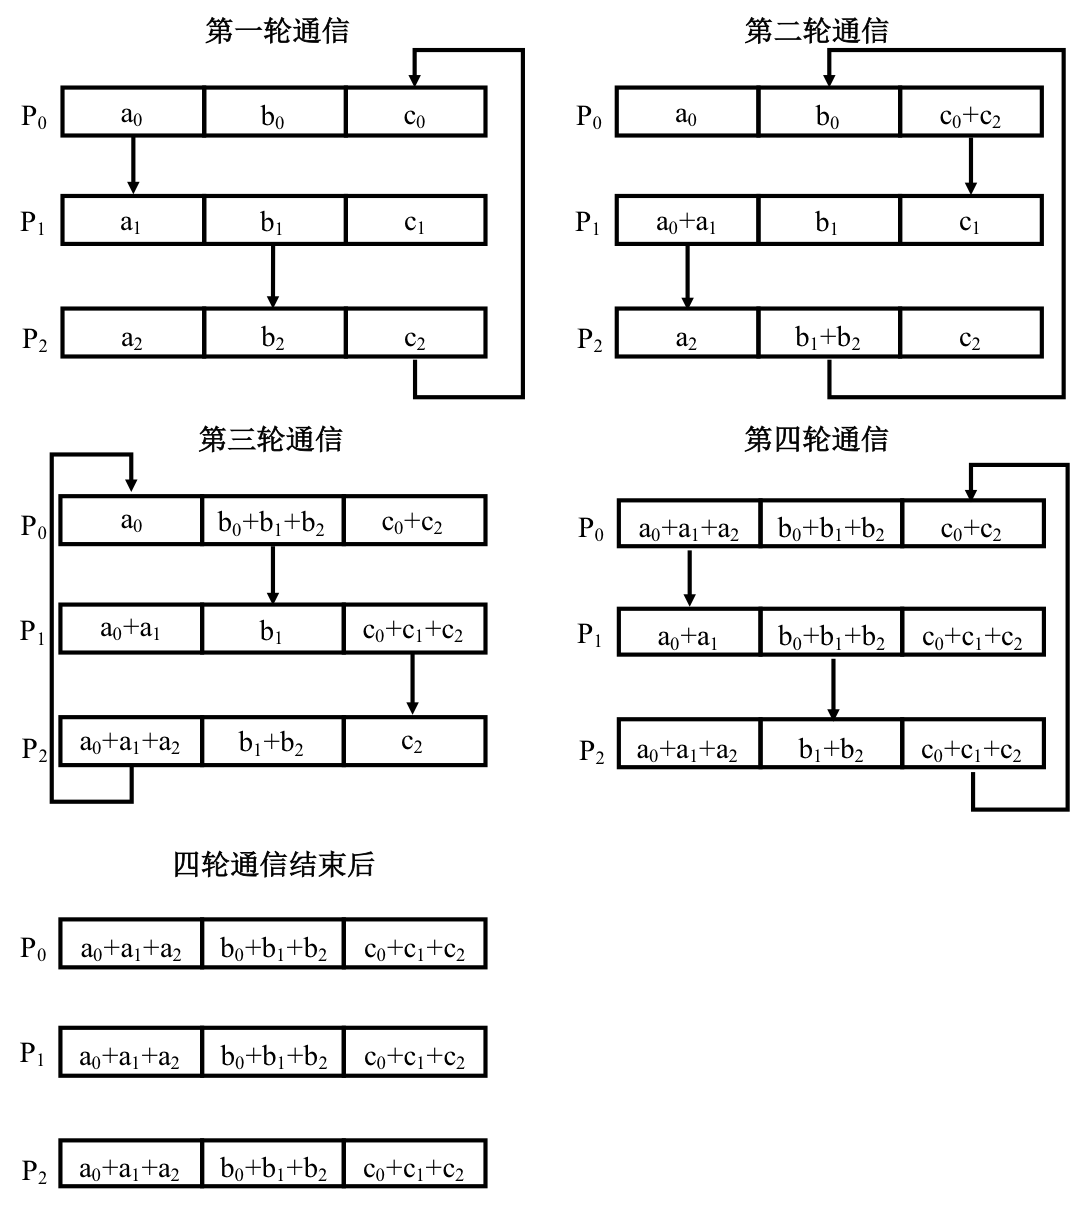
\includegraphics[width = 15cm]{ring-allreduce.png}
    \caption{环形Allreduce算法}
    \label{fig:ring-allreduce}
\end{figure}

\begin{figure}[ht] % use float package if you want it here
    \centering
    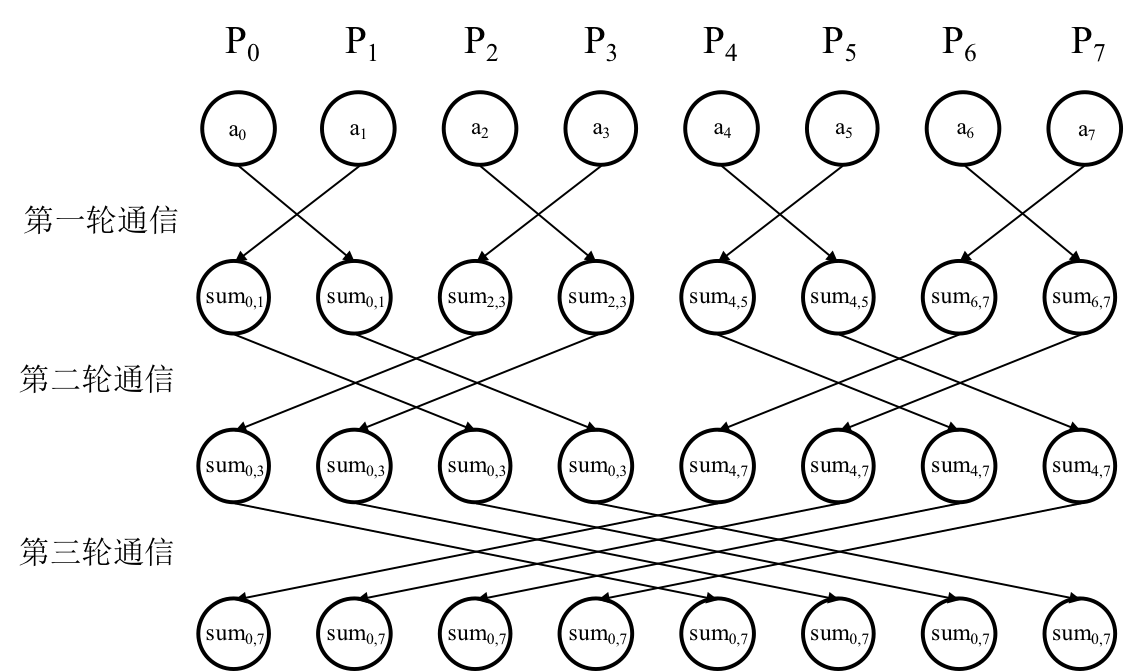
\includegraphics[width = 15cm]{butterfly-allreduce.png}
    \caption{蝶形Allreduce算法}
    \label{fig:butter-allreduce}
\end{figure}


环形算法与蝶形算法的示意图分别如图\ref{fig:ring-allreduce}和图\ref{fig:butter-allreduce}所示,其中,$sum_{l,r}$表示$\sum_{i = l}^r a_i$。环形算法具有通信总量少的优点,而蝶形算法具有通信轮数少的优点。两种算法的对比如表\ref{tab:Allreduce}所示。其中,P为进程数,L为缓冲区长度,并只考虑P为2的整数次幂的情况。

\begin{table}[htb]
    \centering
    \caption[环形算法与蝶形算法对比]{环形算法与蝶形算法对比}
    \label{tab:Allreduce}
    \begin{tabularx}{\linewidth}{lXXX}
        \toprule[1.5pt]
        {Allreduce算法} & {通信轮数} & {单进程每轮通信量} & {单进程通信总量}\\\midrule[1pt]
        环形算法 & $2 \times P - 2$ & $\frac{2 \times L}{P}$ & $ \frac{4 \times (P - 1)\times L}{P}$\\
        蝶形算法 & $log_2(P)$ & $2\times L$ & $2 \times L \times log_2(P)$\\
        \bottomrule[1.5pt]
    \end{tabularx}
\end{table}

\section{随机选择算法}
有一类问题:给定一个包含n个数值的数组,需要从这n个值中选择出第k大的值。我们称此类问题为第k大值问题。深度梯度压缩技术需要选择出绝对值最大的一部分梯度,这和第k大值问题是等价的,因为只需要选出第k大梯度,再找出比第k大梯度更大的梯度即可。

随机选择算法\cite{IntroToAlgo}可以在期望$\Theta(n)$的时间内解决该问题。

如同快速排序算法,随机选择算法的思想也是对输入的数组进行递归划分,不过与快速排序算法不同的是,随机选择算法只选择划分的一侧进行递归,而快速排序算法会在划分的两侧都进行递归。

以下是随机选择算法的伪代码,它返回数组a[l..r]中的第k大的元素。


\makeatletter
\newenvironment{breakablealgorithm}
  {% \begin{breakablealgorithm}
   \begin{center}
     \refstepcounter{algorithm}% New algorithm
     \hrule height.8pt depth0pt \kern2pt% \@fs@pre for \@fs@ruled
     \renewcommand{\caption}[2][\relax]{% Make a new \caption
       {\raggedright\textbf{\ALG@name~\thealgorithm} ##2\par}%
       \ifx\relax##1\relax % #1 is \relax
         \addcontentsline{loa}{algorithm}{\protect\numberline{\thealgorithm}##2}%
       \else % #1 is not \relax
         \addcontentsline{loa}{algorithm}{\protect\numberline{\thealgorithm}##1}%
       \fi
       \kern2pt\hrule\kern2pt
     }
  }{% \end{breakablealgorithm}
     \kern2pt\hrule\relax% \@fs@post for \@fs@ruled
   \end{center}
  }
\makeatother
%\begin{algorithm}[H]
\begin{breakablealgorithm}
\begin{algorithmic}[1]
\Procedure{RANDOMIZED-SELECT}{$a, l, r, k$}
\State $k \gets r - l - k + 2$
\If {$ l=r$}

\Return $a[l]$
\EndIf
\State $q \gets $ \Call{RANDOMIZED-PARTITION}{$a, l, r$}
\State $tmpK \gets q - l + 1$
\If {$ k = tmpK$}

\Return $a[q]$
\ElsIf {$k < tmpK$}

\Return \Call{RANDOMIZED-SELECT}{$a, l, q-1, k$}
\Else

\Return \Call{RANDOMIZED-SELECT}{$a, q+1, r, k-tmpK$}
\EndIf
\EndProcedure
\end{algorithmic}
%\end{algorithm}
\end{breakablealgorithm}

随机算法中调用了RANDOMIZED-PARTITION函数,它的作用是随机选择a[l..r]中的一个元素作为关键字,将比关键字小的元素都放在关键字左侧(下标小于关键字所在下标),其余元素放在右侧(下标大于关键字所在下标)。其伪代码如下所示,其中,RANDOM(i,j)表示从区间[i,j]中随机选取一个整数,SWAP(a[i], a[j])表示交换a[i]和a[j]的值.

\makeatletter
\newenvironment{breakablealgorithm2}
  {% \begin{breakablealgorithm}
   \begin{center}
     \refstepcounter{algorithm}% New algorithm
     \hrule height.8pt depth0pt \kern2pt% \@fs@pre for \@fs@ruled
     \renewcommand{\caption}[2][\relax]{% Make a new \caption
       {\raggedright\textbf{\ALG@name~\thealgorithm} ##2\par}%
       \ifx\relax##1\relax % #1 is \relax
         \addcontentsline{loa}{algorithm}{\protect\numberline{\thealgorithm}##2}%
       \else % #1 is not \relax
         \addcontentsline{loa}{algorithm}{\protect\numberline{\thealgorithm}##1}%
       \fi
       \kern2pt\hrule\kern2pt
     }
  }{% \end{breakablealgorithm}
     \kern2pt\hrule\relax% \@fs@post for \@fs@ruled
   \end{center}
  }
\makeatother
%\begin{algorithm}[H]
\begin{breakablealgorithm}
\begin{algorithmic}[1]
\Procedure{RANDOMIZED-PARTITION}{$a, l, r$}
\State $i \gets$ \Call{RANDOM}{$l, r$}
\State \Call{SWAP}{$a[r], a[i]$}
\State $x \gets a[r]$
\State $i \gets l - 1$
\For{$j \gets l$ to $r -1$}
\If{$a[j] <= x$}
\State $i \gets i + 1$
\State \Call{SWAP}{$a[i], a[j]$}
\EndIf
\EndFor
\State \Call{SWAP}{$a[i+1],a[r]$}
\State \Return $i + 1$
\EndProcedure
\end{algorithmic}
%\end{algorithm}
\end{breakablealgorithm}

\section{智能网卡}
智能网卡与标准网卡的主要区别在于智能网卡有相对较强的计算能力,它可以从主机端处理器卸载计算量。标准网卡的功能只有收发数据包、帧的拆封与封装等,而对于智能网卡而言,程序员可以在上面编程,使网卡可以处理更复杂的计算。

智能网卡主要基于两种技术解决方案,一种是现场可编程门阵列,另一种是中央处理器。

目前,智能网卡的主要应用包括数据包过滤(比如格式验证或分类),数据包转换(比如串行化、压缩或加密)、数据包引导(比如中央处理器核的负载平衡)以及数据包生成等。
\chapter{一种面向稀疏矩阵的Allreduce优化技术}
\label{chap3}

\section{动机}

随着神经网络技术的不断发展,尤其是ResNet~\cite{he2016deep}与BERT~\cite{devlin2018bert}网络的出现,深度神经网络的设计逐渐向着网络更深且参数更多的方向发展,因为这样的网络可以得到更高的精度。但是随着网络变大,训练网络所需要的时间也就变得更长。

为了缩短训练时间,就需要使用多块显卡同时训练,甚至需要用多台机器进行分布式训练。由于深度神经网络训练的特殊性,导致其计算与通信难以重叠,网络带宽也就成为了深度神经网络分布式训练的一处瓶颈。随着多台计算设备的引入,同一个网络在相同训练集上的计算速度可以得到很大的提升,但不幸的是,神经网络相关的数据(尤其是梯度)在显卡之间以及机器之间相互传输花费了大量的时间,分布式训练的并行效率并不高。在网络环境较差的条件下(比如一些实验室只有以太网),深度神经网络的分布式训练的计算--通信比甚至低于50\%。

为了减少深度神经网络分布式训练中通信的开销,最近几年有很多新算法与新网络被提出,包括梯度压缩~\cite{han2015deep},深度梯度压缩~\cite{lin2017deep},以及一些与联合学习有关的算法~\cite{konevcny2016federated, mcmahan2016communication}等。这些算法与网络的核心思想都是在不改变原深度神经网络结构且保持精度不下降(或稍微下降)的前提下,减少分布式训练中需要传输的通信量。

深度梯度压缩技术通过只选取深度神经网络反向传播算法所得到的梯度中的最重要的——即绝对值最大的——0.1\%的参数进行传输,也能够保持最终神经网络训练所得到的精度基本不变。得益于通信量的大幅度减少,分布式训练的时间也随之减少,训练速度得到一定提升。
但是深度梯度压缩技术的实现还有一些方面存在一定问题,具有继续优化的空间。

\subsection{环形Allreduce算法的性能问题}
  在大多数深度学习网络框架内,分布式训练在通信阶段使用的Allreduce算法为环形算法(比如Pytorch的官方后端Gloo中所使用的就是环形Allreduce算法)。
  
  在第\ref{section:MPI-Allreduce}节我们分析过,环形算法拥有总通信量非常小的优点,但是相对的,其通信轮数非常多。在深度神经网络参数较多、通信量较大时,环形算法确实有着非常大的优势。但是若通信量较小,那么环形算法就无法体现出自己的优势,因为此时通信的瓶颈不在网络带宽,而在网络延迟,又由于环形算法的通信轮数较多,引入了较大的延迟,反而会不如其他Allreduce算法。由于环形算法的通信轮数与节点数成正相关,所以节点数越多时,环形算法在通信量较小的传输中的劣势也就越大。
  
  所以对于使用了深度梯度压缩技术的深度神经网络分布式训练而言,使用传统深度学习框架后端的环形Allreduce算法并不合适。

\subsection{稀疏矩阵压缩与解压缩的开销}
使用深度梯度压缩技术后,只需要将梯度中0.1\%参数进行通信。梯度矩阵只有0.1\%的非零元,非常稀疏,所以会进行压缩并采用稀疏矩阵的格式进行传输。

在Allreduce操作中,每完成一轮传输,都需要用接收到的数据与本地数据进行加法操作,即逐元素地将两者对应位置的每一个元素分别相加。但由于采用了稀疏矩阵的格式,无法直接按位相加。

若在每一轮接收到稀疏矩阵格式的数据后,先将其解压缩为一个普通矩阵,再进行逐元素的加法操作,之后再压缩为稀疏矩阵,再进行下一轮的传输,这样会非常的浪费时间。
%如表(这里需要插入一个表格),在对一个大小为2GB的矩阵(512M个单精度浮点数)进行一轮的Allreduce操作中,(应该在表格注明单线程)压缩、解压缩与Reduce操作各需要xxxx秒、xxxx秒和xxxx秒,而稀疏矩阵通信仅需要xxxx,大部分的时间都用在压缩、解压缩与Reduce操作。
若能设计一种算法,使得逐元素的按位加法操作可以在稀疏矩阵格式下直接进行,就可以省去每轮中压缩与解压缩的时间,同时,也可以省去按位相加时大量没有意义的零元加法的时间。
%(这里可以加一张图,两个矩阵大量零元,两个零相加是冗余的用颜色标注出来)

\subsection{设备间的传输延迟}
如图\ref{fig:topology}是两个节点通信的拓扑结构图。若使用标准网卡,每一轮通信都需要先由一台机器将稀疏矩阵由内存发送至网卡,网卡再通过网络(也许中间会经过交换机等设备)发送至其他机器的网卡,其他机器再将数据由网卡发送至内存。

\begin{figure}[ht] % use float package if you want it here
  \centering
  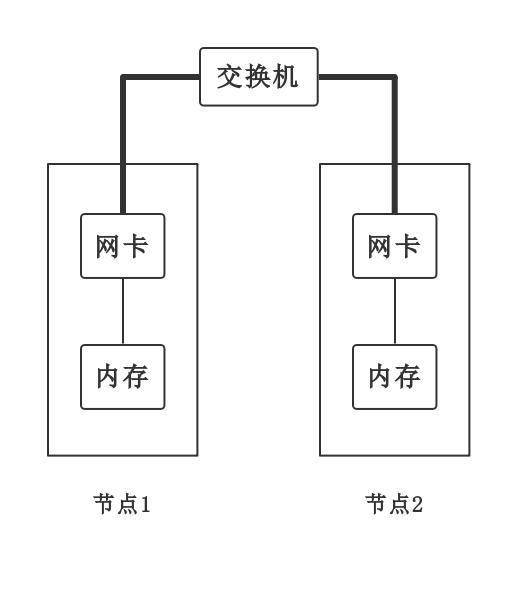
\includegraphics[width = 10cm]{topology.jpeg}
  \caption{两节点通信拓扑结构图}
  \label{fig:topology}
\end{figure}

根据上一节的分析,若算法可以在稀疏矩阵格式下直接进行按位加法操作,其计算量是非常小的,Allreduce的瓶颈主要在各设备之间的通信延迟。由于计算量较小,并不需要计算性能很高的CPU或GPU设备,所以在接下来本文设计的算法中可以使用智能网卡。智能网卡的引入可以避免每轮传输中机器内部从内存到网卡的两次传输延迟,即每轮通信只发生在网卡与交换机之间(图\ref{fig:topology}中的加粗部分),主机端内存并不参与其中。并且由于稀疏矩阵加法的计算量非常小,即使智能网卡上的CPU性能没有主机端的CPU性能高,也并不会导致产生过多的额外计算时间。

\section{算法设计}
\subsection{稀疏矩阵的存储格式}
\label{subsec:sparse-format}
%可以考虑在第二章介绍一下稀疏矩阵存储格式
%在前文中(引用)我们介绍过多种稀疏矩阵的存储格式,但它们都不太适合稀疏的神经网络梯度矩阵的通信。
在大多数深度学习框架中,神经网络的每一层参数都存储在连续的内存中,在进行分布式训练的反向传播时,它们会计算出网络中每一层参数的梯度,等整个网络的梯度都计算完成后,将每层的梯度拼接在一起,形成一个完整且连续的梯度矩阵。与其说是梯度矩阵,不如说成是梯度向量会更合适,因为它们在内存中是连续的。

经典的稀疏矩阵存储格式,如CSC,CSR等,它们能高效地存储二维矩阵,但对于一维的向量而言,反而会带来不必要的存储开销。所以本文选择了更适用于一维稀疏向量且能够支持稀疏格式下的直接加法的存储格式。

可以将这种存储格式抽象为:
[($index_0$, $val_0$), ($index_1$, $val_1$), ($index_2$, $val_2$), $\cdots$, ($index_{n-1}$, $val_{n-1}$)]。

其中,$index_i$表示表示第i个非零元在矩阵按行展开后的位置,也就是相对于矩阵在内存中的起始地址而言,第i个非零元在内存中的相对位置;而$val_i$则表示第i个非零元的数值。

\begin{figure}[ht] % use float package if you want it here
  \centering
  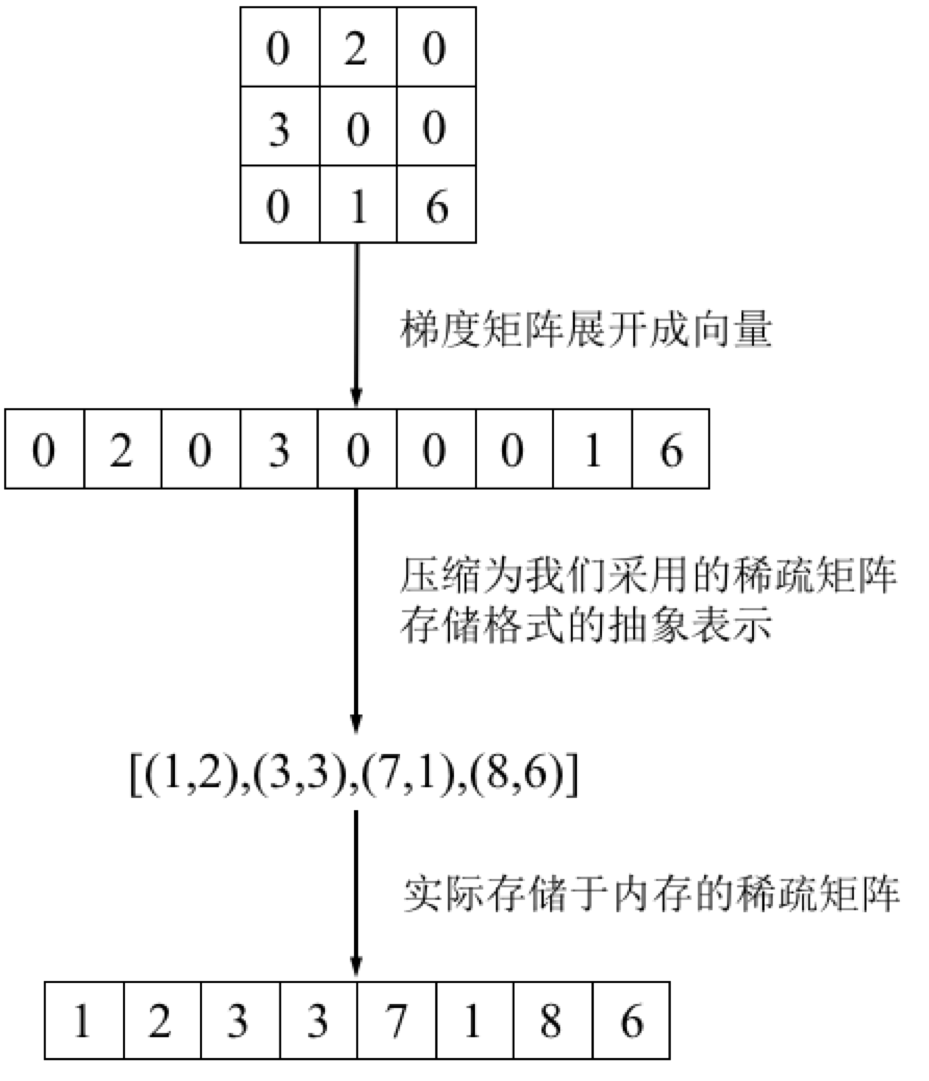
\includegraphics[width = 11cm]{sparse-format.png}
  \caption{稀疏矩阵的存储格式}
  \label{fig:sparse-format}
\end{figure}

在图\ref{fig:sparse-format}中可以更形象、清楚地看出本文所采用的存储格式的实际含义。在实际应用中,梯度矩阵中存储的都是浮点数,但是为了方便,在本文中将以整数的形式表示。

\subsection{稀疏矩阵的加法}
本文设计的稀疏格式下的加法算法的思想类似于归并排序,不过是以index为关键字而不是以val为关键字。算法伪代码如下,输入为两个稀疏矩阵和它们的非零元个数:
\makeatletter
\def\BState{\State\hskip-\ALG@thistlm}
\makeatother
\begin{algorithm}
\begin{algorithmic}[1]
\Procedure{SPARSE-ADDITION}{$src_0, src_1, num_0, num_1$}
\State $index_0 \gets 0$
\State $index_1 \gets 1$
\For{$i \gets 0 $ to $num_0 + num_1 - 1$}
\If{$index_1 >= num_1$ \textbf{or} $src_0[index_0].index < src_1[index_1].index$}
\State $dst[i].index \gets src_0[index_0].index$
\State $dst[i].value \gets src_0[index_0].value$
\State $index_0 \gets index_0 + 1$
\ElsIf{$index_0 >= num_0$ \textbf{or} $src_0[index_0].index > src_1[index_1].index$}
\State $dst[i].index \gets src_1[index_1].index$
\State $dst[i].value \gets src_1[index_1].value$
\State $index_1 \gets index_1 + 1$
\ElsIf{$src_0[index_0].index = src_1[index_1].index$}
\State $dst[i].index \gets src_0[index_0].index$
\State $dst[i].value \gets src_0[index_0].value + src_1[index_1].value$
\State $index_0 \gets index_0 + 1$
\State $index_1 \gets index_1 + 1$

\EndIf
\EndFor
\State \Return $dst$
\EndProcedure
\end{algorithmic}
\end{algorithm}


如图\ref{fig:sparse-addition}为稀疏矩阵加法的示意图。

\begin{figure}[ht] % use float package if you want it here
  \centering
  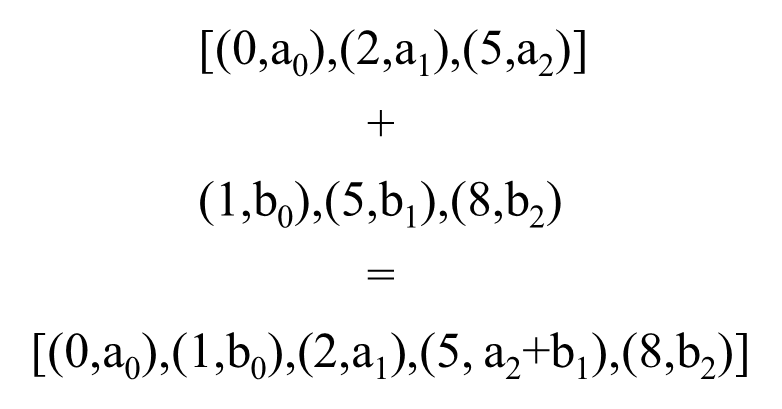
\includegraphics[width = 11cm]{sparse-addition.png}
  \caption{稀疏矩阵的加法}
  \label{fig:sparse-addition}
\end{figure}

前文提到,这个算法类似于归并排序,且是以index作为关键字。这实际上对应着本文设计的算法需要满足的一条重要的性质:输入的两个稀疏矩阵中的index必须是有序的。这就类似于在归并排序中,需要进行归并的两个数组中的元素必须是有序的一样。只有输入的两个稀疏矩阵中的index有序,才能够保证算法的正确性;换句话说,如果index无序的话,就无法正确的将两个index相同的val正确地进行合并。

幸运的是,根据算法流程,只要输入的两个稀疏矩阵中的index是有序的,输出的稀疏矩阵中的index也将会是有序的。这也就意味着,只需要确保所有梯度矩阵在压缩时可以按照index的顺序进行压缩,之后所有轮次中的稀疏矩阵相加的正确性就是有保证的,这可以使用数学归纳法进行证明。

有了稀疏矩阵的加法,就可以只在Allreduce算法的最开始进行一次梯度矩阵的压缩,且只在Allreduce算法结束前进行一次稀疏矩阵的解压缩,在Allreduce算法的每一轮中不需要再进行压缩或解压缩,直接进行稀疏矩阵的加法即可,这大大缩短了Allreduce算法的执行时间。

同时,稀疏矩阵的加法避免了普通按位Reduce操作中,由于梯度矩阵过于稀疏而导致的大量冗余的零元加法。

\subsection{Allreduce算法选择}
在本文的算法中,Allreduce的每一轮通信都是传输一个稀疏矩阵,相对于传统深度学习分布式训练的多机通信而言,本文的算法通信量并不大。

随着通信量的减少,通信部分的瓶颈不在网络带宽,而在网络延迟。拥有“总通信量少”的特点的环形Allreduce算法将不再具有优势,同时,环形算法的“轮数多”的特点将会使得网络延迟更为严重。大多数深度学习框架所采用的环形Allreduce算法对于本文而言并不合适。

本文选择使用蝶形算法,在进程数为n时,蝶形算法只需要用$\lceil log_2(n) \rceil$轮就可以完成Allreduce算法。虽然蝶形算法的总通信量较大,但由于通信的是比较小的稀疏矩阵,所以这并不会为Allreduce算法带来较多的额外通信时间。

\subsection{使用智能网卡降低设备传输延迟}
综合前文所述,现在可以把本文所设计的算法流程概括如下(为方便起见,只考虑进程数为2的正整数次幂的情况。算法轮数从0开始计数,进程数从0开始计数,每台机器只启动一个进程执行分布式训练):
\begin{itemize}
  \item [1)]
  进程将梯度矩阵输入进随机选择算法,选出梯度矩阵中第$\frac{size}{1000}$大的浮点数作为阈值,其中,size为梯度矩阵中浮点数的个数。
  \item [2)] 
  通过随机选择法得到的阈值,筛选出稠密度为$\frac{1}{1000}$的矩阵,并将其压缩成第\ref{subsec:sparse-format}节中描述的稀疏矩阵格式,将得到的稀疏矩阵设置为本地稀疏矩阵。
  \item [3)]
  在算法的第i轮,第x台机器与第x xor $2^i$台机器进行通信,这两台机器别将自己的本地稀疏矩阵发送给对方,并从对方接收对方发送来的的稀疏矩阵。
  \item [4)]
  将自己的本地稀疏矩阵与接收的对方的稀疏矩阵进行稀疏矩阵加法,将加法得到的矩阵再次设置为本地稀疏矩阵。
  \item [5)]
  重复过程3)$\sim$4),直到$log_2(n)$轮的蝶形算法完成。
  \item [6)]
  将本地稀疏矩阵解压缩为梯度矩阵,用于更新模型参数。
\end{itemize}

若要更细粒度地、从设备的角度分析Allreduce算法的通信过程,可以将过程3)扩充如下:
\begin{itemize}
  \item [3.1)]
  存储于每一台机器内存中的本地稀疏矩阵被传输到机器的网卡内。
  \item [3.2)]
  第x台机器的网卡与第x xor $2^i$台机器的网卡之间通过交换机等设备进行通信,这两台机器的网卡别将自己的本地稀疏矩阵发送给对方网卡,并从对方接收对方发送来的的稀疏矩阵。
  \item [3.3)]
  每台机器将网卡接收到的稀疏矩阵发送至机器内的内存。
\end{itemize}

根据前文分析,由于本文所采用算法的通信量较少,通信的瓶颈在延迟,降低传输延迟就能够有效缩短算法执行时间。为了能够降低通信延迟,本文已经使用了通信轮数更少的Allreduce算法,若要想进一步降低通信延迟,还可以减少参与一轮通信的设备数。

若使用标准网卡进行通信,如3.1)$\sim$3.3)所描述的那样,每轮通信所要经过的设备是内存$\rightarrow$网卡$\rightarrow$交换机$\rightarrow$网卡$\rightarrow$内存。若使用具有计算功能的智能网卡,就可以将稀疏矩阵加法放在网卡上进行计算,主机端中央处理器不再需要进行稀疏矩阵的加法,每轮通信也就不再需要将信息发送至主机端内存。这样可以将参与每轮通信的设备缩减至网卡$\rightarrow$交换机$\rightarrow$网卡。

尽管智能网卡上的中央处理器的计算性能不如主机端的中央处理器,但是用于计算稀疏矩阵的加法还是绰绰有余的。稀疏矩阵加法的计算量并不大,它并不是一个计算密集型任务,在接下来的实验中我们也将看到,稀疏矩阵加法是各项操作中(包括压缩、解压缩、第k大梯度选择以及稀疏矩阵通信)耗时最短的。所以使用性能较差的网卡上的中央处理器进行稀疏矩阵加法也并不会在计算上引入过多的额外时间,反而能够通过不将稀疏矩阵与主机端的内存进行通信而达到降低传输延迟的效果。

不过相比于计算量较少的稀疏矩阵加法,对于压缩和解压缩这种计算量较大的操作,还是更适合放在主机端中央处理器来进行计算。也就是说,若使用智能网卡,则在Allreduce算法的最开始,由主机端中央处理器将梯度矩阵压缩成稀疏矩阵,并将其发送至智能网卡。之后Allreduce的每轮通信与稀疏矩阵加法都只在各个智能网卡之间进行,不经过主机端中央处理器和内存。等Allreduce算法的所有轮通信都执行完之后,智能网卡再将稀疏矩阵发送至主机端内存,并由主机端中央处理器将其解压缩至梯度矩阵。

\subsection{第k大梯度选择的优化}
\label{subsec:topKOptimize}
前文中我们介绍过随机选择算法,该算法可以在期望$\Theta(n)$的时间内找到n个元素的数组中第k大的数值。

虽然随机选择算法的计算复杂度较低,且算法主体的访存是连续的,对cashe比较友好,但是算法常数仍然比较大,执行速度较慢。经分析,其原因主要是在随机选择算法的RANDOMIZED--PARTITION函数中,有大量的条件判断语句将一个数组中的元素与固定的关键字进行比较。由于关键字是从所有数值中随机选择出来的,所以任何一个数值与关键字的大小关系是随机的,这就导致了中央处理器的分支预测技术预测出的分支结果的正确率非常低(平均只有50\%)。又由于分支预测失败后的开销较大,所以随机选择算法的常数比较大。遗憾的是,由于随机选择算法本身设计,这种分支预测的失败是无法避免的。

同时,随机选择算法的RANDOMIZED--PARTITION部分几乎无法使用多线程等方法来通过并行计算取得加速效果,所以随机选择算法本身几乎无法优化。

既然随机选择算法难以优化,且随机选择算法的执行时间又与输入算法的数据量有关,那么若想要减少随机选择算法的执行时间,一个很直观的想法就是减少输入随机选择算法的数据量。若减少了输入随机选择算法的数据量,为了保证算法的正确性,也就是随机选择算法能够正确的选择出原梯度矩阵中所有数值的第$\frac{size}{1000}$大的数值,而不是输入随机选择算法中的第$\frac{n}{1000}$大的数值\footnote{size为原梯度矩阵中浮点数的个数,n为输入随机选择算法的浮点数的个数},也就需要保证,原梯度矩阵中的前$\frac{size}{1000}$大的所有数值,都要被输入随机选择算法。

为了找出原梯度矩阵中的前$\frac{size}{1000}$大的所有数值,就需要用一个数值作为阈值去筛选原梯度矩阵,这个阈值必须要比前$\frac{size}{1000}$大的数值小,但是由于之后要将筛选出的数值输入随机选择算法,所以为了随机选择算法执行时间更短,就需要让被筛选出的数值尽量少,或者说,需要让阈值在比前$\frac{size}{1000}$大的数值小的同时尽量大。为了得到这样的一个阈值,本文采用的方法就是先采样,再调用随机选择算法。

本文设计的第k大梯度选择的算法流程如下:
\begin{itemize}
  \item [1)]
  设置k大值比例topK\_ratio为0.5\%。
  \item [2)]
  对原梯度矩阵进行采样,采样共$\frac{size}{100}$个数值,将它们输入至随机选择算法,选择出它们中的第$\frac{size}{100}\times sample\_ratio$大的数值作为阈值。
  \item [3)]
  使用阈值对原梯度矩阵进行筛选,将大于阈值的梯度筛选出来。
  \item [4)]
  将被筛选出的梯度的数量与$\frac{size}{1000}$进行比较,若被筛选出的梯度的数量小于$\frac{size}{1000}$,则说明选择的阈值大于原梯度矩阵中第$\frac{size}{1000}$大的梯度,需要重新选择阈值。为了使阈值更大,就将k大值比例变为原来的两倍,即$topK\_ratio = topK\_ratio \times 2$,并跳转到2)继续执行;直到被筛选出的梯度的数量大于或等于$\frac{size}{1000}$。
  \item [5)]
  将被筛选出的梯度输入随机选择算法,选出它们中的第$\frac{size}{1000}$大的数值。
\end{itemize}

算法中的采样的梯度对选出来的阈值有很大影响。若采样的梯度整体偏大,则选出的阈值也会比较大,反之亦然。在理想情况下,原梯度矩阵分布均匀,采样的梯度也就可以代表原梯度矩阵,所选出的阈值也会比较合适,即在比前$\frac{size}{1000}$大的梯度小的同时尽量大。但是实际上,在神经网络反向传播中,梯度的分布并不会非常均匀。为了使得采样尽量均匀,我们会在梯度矩阵中选择多处位置,每一处采样连续的一段梯度,然后将各处的采样拼接到一起,作为最终的采样结果输入值随机选择算法。

但是,即使采用了这种尽量均匀的采样方式,采样得到的梯度分布也依然不会和原梯度矩阵的分布是一样的。若根据采样梯度选出的阈值比原梯度矩阵中第$\frac{size}{1000}$大的梯度还要大的话,之前所选出来的阈值就没有任何意义,随机选择算法所消耗的时间也将白白浪费。所以,提高选出可用的阈值的概率,我们将随机选择算法要选择的k大值的比例由0.1\%提高到0.5\%。这样一来,即使采样并不够均匀,但是采样的梯度中第$\frac{sample\_size}{200}$大的梯度\footnote{sample\_size为采样的梯度数量,即$\frac{size}{100}$}很大概率上还是会小于原梯度矩阵中第$\frac{size}{1000}$的梯度。

即使有了选取多段采样以及提高k大值的比例这两项措施,随机选择算法选出的阈值仍然可能不满足小于原梯度矩阵中第$\frac{size}{1000}$大梯度的要求。这时,算法会再次提高k大值的比例,重新采样并调用随机选择算法选取阈值,直到选取出满足条件的阈值为止。

这个算法流程虽然看似步骤繁多,但这并不会使得算法执行时间较长,因为算法的每一步设计的数据量比较小。比如采样并输入进随机选择算法的梯度只有原梯度矩阵的1\%,并且在平均情况下,通过阈值筛选出来并输入随机选择法算法的梯度只有原梯度矩阵的0.5\%。而在前文中提到了随机选择算法的时间复杂度为$\Theta(n)$,那么相比于将原梯度矩阵全部输入进随机选择算法,通过对梯度矩阵的处理,随机选择算法的执行时间将只有原来的1.5\%左右。

算法中最耗时的部分是使用阈值筛选原梯度矩阵,这一步需要遍历梯度矩阵中所有梯度。不过,在平均情况下,算法选出的阈值会大于梯度矩阵中99.5\%的梯度,所以中央处理器的分支预测会有极高的准确率,代码执行速度也会非常快。经过测试,在单线程下,与使用原梯度矩阵直接调用随机选择算法相比,经过本文优化后的第k大梯度选择过程的速度提高了13.3倍。

同时,最耗时的筛选过程可以使用多线程进行并行计算,这样就能进一步缩短算法执行时间。

\subsection{算法总述}
本文从四个方面对稀疏矩阵的Allreduce过程进行优化,如图\ref{fig:summary}所示。

\begin{figure}[ht] % use float package if you want it here
  \centering
  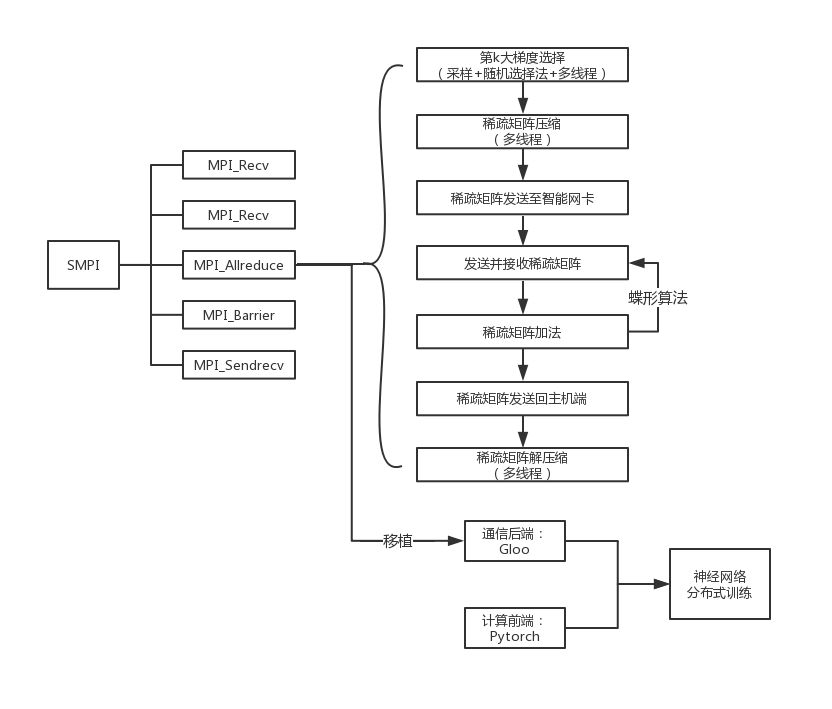
\includegraphics[width = 15cm]{summary.png}
  \caption{算法总述}
  \label{fig:summary}
\end{figure}

在本文提出的优化算法中,首先使用基于采样的方法,通过多次调用随机选择算法来对第k大梯度的选择过程进行加速。根据选择出的阈值,再将梯度矩阵压缩为稀疏矩阵。之后将稀疏矩阵发送至智能网卡,并在智能网卡之间执行蝶形算法。蝶形算法的每一轮,智能网卡会先发送并接受稀疏矩阵,之后在智能网卡上直接进行稀疏矩阵的加法,不需要压缩与解压缩操作。蝶形算法只发生在智能网卡之间,主机端并不参与其中。蝶形算法结束后,智能网卡将稀疏矩阵再发送至主机端,由主机进行稀疏矩阵的解压缩。对于第k大梯度选择与稀疏矩阵的压缩和解压缩过程,本文都使用了多线程并行计算。
\chapter{实验}
\label{chap4}

\section{实验设计}
我们的实验主要分为两部分:
\begin{itemize}
    \item 与OpenMPI对比,测试我们设计的Allreduce算法的性能。
    \item 将我们的算法移植至深度学习框架,使用真实数据集进行分布式训练,测试训练性能。
\end{itemize}

为了测试我们的Allreduce算法的性能,我们实现了一个简单的MPI库---SMPI。SMPI内实现了多种MPI原语:
\begin{itemize}
    \item MPI\_Send()
    \item MPI\_Recv()
    \item MPI\_Sendrecv()
    \item Barrier()
    \item Allreduce()
\end{itemize}

SMPI支持两种模式:普通模式与智能网卡模式。处于智能网卡模式下的SMPI,在Allreduce算法的开始会先在主机端中央处理器进行第k大梯度选择并将梯度矩阵压缩为稀疏矩阵格式,再将稀疏矩阵传送至智能网卡;之后的每轮通信都发生在各个智能网卡之间,同时,稀疏矩阵加法也在智能网卡上进行;所有轮次的通信结束后,智能网卡将稀疏矩阵重新发回至主机端中央处理器并将稀疏矩阵重新解压缩为梯度矩阵,继续进行反向传播算法。处于普通模式下的SMPI,则没有那么复杂,所有计算都是在主机端中央处理器进行的,网卡仅用于通信,且主机端并不需要与网卡显示通信,换句话说,网卡对于普通模式下的SMPI而言是透明的。

目前,SMPI只支持使用TCP进行通信。

我们使用了OpenMPI作为基线与SMPI进行对比。OpenMPI支持使用TCP或RDMA进行通信。

在这之后,我们使用深度学习框架Pytorch,将我们的算法移植至Pytorch的后端---Gloo\footnote{Gloo是facebook的一个孵化项目,也是Caffe2与Pytorch的官方后端。Gloo的源代码在以下网址:https://github.com/facebookincubator/gloo。},并选择了几个神经网络模型,输入真实的数据集进行分布式训练以测试我们的Allreduce算法所带来的分布式训练的性能提升。

我们选择的数据集是Cifar10~\cite{krizhevsky2009learning}数据集,它包含50000张训练集图片以及10000张验证集图片,图片共有10个类别。

我们的工作主要关注神经网络的分布式训练速度,至于训练出的模型能够达到的精度,我们并没有进行测试。这并不代表我们训练出的模型精度不高,而是由于我们的工作是基于深度梯度压缩技术,并且没有从算法的根本原理上改变深度梯度压缩技术。换句话说,我们的算法能够提高分布式训练的速度,但是算法得到的稀疏梯度矩阵与原深度梯度压缩所得到的稀疏矩阵是相同的,我们的算法并不会影响反向传播过程中模型参数的更新。所以,使用我们的优化算法得到的模型精度与直接使用深度梯度压缩技术得到的模型精度是相同的。

我们的SMPI代码与移植后的Gloo代码都已开源\footnote{SMPI的代码位于https://github.com/sth1997/smpi,移植后的Gloo代码位于https://github.com/sth1997/gloo。}。

\section{实验平台}
本次实验使用了8台服务器,每台服务器的中有2个Intel XeonE5-2670 v3 处理器,每个中央处理器有12个物理核心,其主频为2.3GHz,并支持超线程技术,共有24线程。每台服务器拥有128GB内存。

8台服务器所组成的集群使用1000Mb Ethernet与100Gb Infiniband连接。

服务器中安装的操作系统为Ubuntu 16.04.4 LTS。实验中使用的OpenMPI版本为4.0.0,使用的Pytorch版本为1.2.0a0+81e70ff,使用的Gloo版本为0.5.0。

我们所使用的智能网卡为Mellanox BlueField,它上面有2个25Gb Ethernet SFP28 接口,16GB主板上的内存,以及1个具有8个物理核心的Armv8 A72 中央处理器。

\section{实验结果及分析}
\subsection{SMPI Allreduce性能测试}
\chapter{结论}
\label{chap5}

\section{本文的研究内容和结论}
本文以深度梯度压缩技术为基础,并在稀疏矩阵的加法、Allreduce算法选择、第k大梯度选择以及智能网卡的使用等多方面进行优化,最终将稀疏矩阵Allreduce过程性能提升至Open MPI Allreduce过程性能的38.0倍,并将优化了Allreduce过程的Pytorch分布式训练性能提升至原来的8.6倍,这使得即使在使用带宽较低的1000 Mbps Ethernet时,用了本文的算法进行优化,得到的性能依然可以比肩甚至超越使用带宽较高的100 Gbps Infiniband时的原算法性能。同时,本文的算法具有非常好的可扩展性。

具体地,深度梯度压缩技术可以在不影响模型精度的情况下,将分布式训练中需要进行传输的参数量但幅度减少,但是传统的深度学习框架中,分布式训练使用的Allreduce算法都是环形算法,它的通信总量非常少,但是通信轮数较多,并不适合通信量少的情况。所以在我们的算法中,我们使用的是蝶形Allreduce算法,它的通信轮数非常少,并且由于需要通信的参数量非常少,所以通信总量并不大。

深度梯度压缩技术提出了将梯度矩阵压缩为稀疏矩阵后再进行传输的思想,若在Allreduce算法的每一轮都进行压缩、传输再解压缩并进行相加,就会耗费太多时间。本文提出了一种稀疏矩阵直接相加的方法,使用本方法就可以在每轮通信时省去压缩和解压缩的时间。

同时,深度梯度压缩技术需要在梯度矩阵中选择出绝对值最大的k个梯度,这就需要调用随机选择算法来找到第k大梯度的值,并用这个值对原梯度矩阵进行筛选并压缩为稀疏矩阵。但是随机选择算法的速度非常慢,我们会先对原梯度矩阵进行采样,只将部分样本输入进随机选择算法,再结果当做阈值对原梯度矩阵进行筛选,将筛选出来的部分梯度再次输入进随机选择算法的到最终结果。这个优化可以在单线程和多线程下分别将第k大梯度的选择过程的速度提高13.3倍和46.0倍。

最后,我们尝试使用智能网卡,使得Allreduce每轮通信过程只在各节点的网卡之间进行,并在网卡上进行稀疏矩阵的计算,主机端并不参与其中,以此来进一步降低延迟。

根据实验结果,在使用TCP进行通信时,我们实现的SMPI通信库的稀疏矩阵Allreduce性能比Open MPI的普通Allreduce性能高38.0倍。对Pytorch的分布式训练进行优化后,我们选择的几个常用的神经网络的分布式训练性能提高了3.3$\sim$8.6倍。

\section{进一步的工作}
本文实现的SMPI通信库以及移植Gloo的工作目前只支持CPU,并不支持GPU。如前文所说,神经网络的计算--通信比越小,优化Allreduce过程后得到的性能提升就越高。所以,之后若将本文的优化算法移植至GPU,相信可以为神经网络分布式训练带来更高的性能提升。

同时,由于硬件原因,在智能网卡的实验中,我们只使用了两个节点,无法证明智能网卡能够降低Allreduce中每轮通信的延迟。希望在未来的工作中能够完成这部分实验。


%%% 其它部分
\backmatter

%% 本科生要这几个索引,研究生不要。选择性留下。
% 插图索引
\listoffigures
% 表格索引
\listoftables
% 公式索引
\listofequations


%% 参考文献
% 注意:至少需要引用一篇参考文献,否则下面两行可能引起编译错误。
% 如果不需要参考文献,请将下面两行删除或注释掉。
\bibliographystyle{thuthesis-numeric}      % 顺序编码制
% \bibliographystyle{thuthesis-author-year}  % 著者-出版年制
%\bibliographystyle{thuthesis-bachelor}     % 本科生参考文献的著录格式
\bibliography{ref/refs}


%% 致谢
% 如果使用声明扫描页,将可选参数指定为扫描后的 PDF 文件名,例如:
% \begin{acknowledgement}[scan-statement.pdf]
\begin{acknowledgement}
  首先,我要衷心感谢我的导师翟季冬老师。在本学年中,翟老师带领我迈入科研的大门,并引导我学习了很多与系统相关的知识。在选题、算法设计与实验中,翟老师也为我提供了很多帮助,在此我要衷心感谢翟老师对我的关心与指导。

  其次,我要感谢王雨田同学。我使用的智能网卡是Mellanox的一款实验性网卡,安装文档非常不全,且没有任何技术性的博客可以看,我们在一起摸索了将近一周才基本安装起来。非常感谢王雨田同学在此期间的帮助。

  最后,我要感谢我的女朋友黄思捷。在我写毕业论文期间,她在画图方面对我提供了很大帮助,也与我一起查找论文中的格式与逻辑错误。
\end{acknowledgement}


%% 附录
\begin{appendix}
\chapter{外文资料的书面翻译}

\title{英文资料的中文标题}

{\heiti 摘要:} 大规模分布式训练需要大量的通信带宽用于梯度交换,这限制了多节点训练的可扩展性,并且需要昂贵的高带宽网络基础设施。随着移动设备上的分布式训练(联合学习)的出现,情况变得更加糟糕,这种训练具有更高的延迟、更低的吞吐量和间歇性的不良连接。本文发现分布式SGD中99.9\%的梯度交换是冗余的,并提出深度梯度压缩(DGC)来大大降低通信带宽。为了在压缩过程中保持准确率,DGC采用了四种方法:动量修正、局部梯度修剪、动量因子掩蔽和预训练。我们已经将深度梯度压缩应用于图像分类、语音识别和语言模型,使用的数据集包括Cifar10、ImageNet、Penn Treebank和Librispeech Corpus。在这些场景下,深度梯度压缩实现了从270$\times$到600$\times$的梯度压缩比而不损失精度,将ResNet--50的梯度大小从97 MB削减到0.35 MB,对于DeepSpeech 从488 MB削减到0.74 MB,深度梯度压缩使得在廉价的1 Gbps以太网上进行大规模分布式训练成为可能,并方便了移动设备上的分布式训练。


\section{引言}
大规模分布式训练提高了更深和更大模型训练的生产效率。同步随机梯度下降(SGD)广泛用于分布式训练。通过增加训练节点的数量和利用数据并行性,可以显著减少对相同大小的训练数据的前向—反向传播的总计算时间。然而,梯度交换成本很高,这使计算时间的节省相形见绌,特别是对于计算与通信比例低的循环神经网络(RNN)。因此,网络带宽成为扩大分布式训练的一个重要瓶颈。当在移动设备上执行分布式训练时,这种带宽问题变得更加严重,例如联合学习。由于更好的隐私和更好的个性化,移动设备上的训练很有吸引力,但一个关键问题是,这些移动设备的网络带宽更低,网络时断时续,移动数据计划昂贵。

深度梯度压缩(DGC)通过压缩梯度来解决通信带宽问题,如图1所示。为了确保不损失精度,DGC在梯度稀疏化的基础上采用动量修正和局部梯度裁剪来保持模型性能。DGC还使用动量因子掩蔽和预训练来克服通信减少而造成的数据过时问题。

我们根据经验验证了深度梯度压缩在多种任务、模型和数据集上的应用:CNN用于图像分类(使用Cifar10和ImageNet),RNN用于语言模型(使用Librispeech Corpus)和语音识别(使用Librispeech Corpus)。这些实验表明,梯度可以压缩到600倍,而不损失精度,这比以前的工作高一个数量级。

\section{相关工作}
研究人员提出了许多方法来克服分布式训练中的通信瓶颈。例如,一旦节点完成反向传播,异步SGD通过移除梯度同步和立即更新参数来加速训练。梯度量化和稀疏化以减少通信数据大小也被广泛研究。

\paragraph{梯度量化}
将梯度量化为低精度值可以降低通信带宽。Seide等人提出了1比特SGD来减小梯度传输数据大小,并在传统语音应用中实现了10倍的加速。Alistarh等人提出了另一种称为QSGD的方法,该方法对模型精度和梯度精度之间进行平衡。与QSGD相似,Wen等人开发了使用3级梯度的TernGrad。这两项工作都证明了量化训练的收敛性,尽管TernGrad只检测了CNN,而QSGD只检测了RNN的训练损失。也有人试图量化整个模型,包括梯度。DoReFa--Net使用1比特权重和2比特梯度。

\paragraph{梯度稀疏化}
Strom提出了阈值量化用来只发送大于预定常数阈值的梯度。然而,这个门槛在实践中很难选择。因此,Dryden等人(2016年)分别选择了固定比例的正梯度和负梯度更新,Aji与Heafield提出梯度下降,以基于绝对值的单一阈值来稀疏梯度。为了保持收敛速度,梯度下降需要增加层归一化。梯度下降节省了99\%的梯度交换,同时导致机器翻译任务中BLEU分数损失0.3\%。同时,Chen等人提出根据局部梯度活动自动调整压缩率,对于全连通层,压缩率约为200倍,对于卷积层,压缩率约为40倍,而在ImageNet数据集上,top--1准确率的下降基本可以忽略不计。

与之前的工作相比,DGC将整个模型的梯度压缩比提高到600倍(所有层的压缩比相同)。DGC不需要额外的层正则化,因此不需要改变模型结构。最重要的是,深度梯度压缩不会导致精度损失。

\section{深度梯度压缩}

\subsection{梯度稀疏化}
我们通过只发送重要的梯度(稀疏更新)来减少通信带宽。我们使用基于梯度绝对值的简单启发式算法:仅传输大于阈值的梯度。为了避免丢失信息,我们在本地积累其余的梯度。最终,这些梯度变得足够大,可以传输。因此,我们立即发送大梯度,但最终会发送所有梯度,如算法1所示。$encode()$函数包含32位非零梯度值和16位游程长度。我们的关电视,局部梯度累积相当于随着时间的推移增加批大小(batch size)。令$F(w)$为我们想要优化的损失函数。同步分布式SGD通过总共N个训练节点执行以下更新:

\begin{equation}
	\label{eq:dsgd}
	F(w) = \frac{1}{\left|\chi \right|} \sum_{x \in \chi} f(x, w), \qquad
	w_{t+1} = w_{t} - \eta \frac{1}{Nb} \sum_{k=1}^{N}\sum_{x \in \mathcal{B}_{k, t}} \triangledown f(x, w_{t})
\end{equation}

其中$\chi$是训练数据集,$w$是网络的权重,$f(x,w)$是根据样本$x$计算的损失,$x$从$\chi$中采样,$\eta$是学习率,$N$是训练节点的数量,对于$1 \leq k \le N$的$B_k$ 是一个在第$t$轮迭代时从$\chi$中采样的长为$N$的迷你批次(mini batch)序列,每个大小为$b$。

考虑展开后的权重$w$中第$i$个位置的权重$w^{(i)}$。经过$T$轮迭代后,我们有:
\begin{equation}
	\label{eq:titer}
	w_{t+T}^{(i)} = w_{t}^{(i)} - \eta T \cdot \frac{1}{NbT} \sum_{k=1}^{N} \left (\sum_{\tau=0}^{T-1}\sum_{x \in \mathcal{B}_{k, t+\tau}} \triangledown^{(i)} f(x, w_{t+\tau}) \right ) 
\end{equation}

等式2表明,局部梯度累积可以被认为是将批大小从$Nb$增加到$NbT$($\tau$上的第二次求和),其中$T$是发送$w^{(i)}$梯度的两次迭代之间的\emph{稀疏更新间隔}的长度。学习率缩放是处理大型迷你批次的常用技术。学习速率$\eta T$和批大小$NbT$中的$T$被抵消,在等式2中自动满足。

\subsection{提高局部梯度累计}
如果不注意的话,当稀疏度非常高时,稀疏更新将极大地影响收敛。例如,算法1对Cifar10数据集造成了超过1.0\%的准确率损失,如图3(a)所示。我们发现动量修正和局部梯度修剪可以缓解这个问题。

\paragraph{动量修正}
动量SGD被广泛用于代替朴素SGD。然而,算法1并不直接应用于带有动量项的SGD,因为它忽略了稀疏更新间隔之间的折扣因子。

随后是在N个训练节点上使用朴素SGD的分布式训练,

\begin{equation}
	\label{eq:msgd}
	u_{t} = mu_{t-1} + \sum_{k=1}^{N}\left( \triangledown_{k,t}\right),\quad  w_{t+1} = w_{t} - \eta u_{t}
\end{equation}

其中$m$是动量,$N$是训练节点的数量,并且$\triangledown_{k,t} =  \frac{1}{Nb} \sum_{x \in \mathcal{B}_{k, t}} \triangledown f(x, w_{t})$。

考虑展开后的权重$w$中的第$i$个位置的权重$w^{(i)}$。在经过$T$轮迭代之后,权重$w^{(i)}$的变化如下所示:

\begin{equation}
	\label{eq:msgd_change}
	w_{t+T}^{(i)} = w_{t}^{(i)} - \eta \left[\cdots +  \left( \sum_{\tau=0}^{T-2} m^{\tau}\right)\triangledown^{(i)}_{k,t+1} + \left( \sum_{\tau=0}^{T-1} m^{\tau}\right)\triangledown^{(i)}_{k,t}\right]
\end{equation}

如果具有动量的SGD直接应用于稀疏梯度场景(算法1中的第15行),更新规则不再等同于等式3,等式3变为:

\begin{equation}
	\label{eq:nomc}
	v_{k,t} = v_{k,t-1} + \triangledown_{k, t},\quad u_{t} = mu_{t-1} + \sum_{k=1}^{N} sparse\left( v_{k, t}\right) ,\quad  w_{t+1} = w_{t} - \eta u_{t}
\end{equation}

其中第一项是训练节点$k$上的局部梯度累积。一旦累计结果$v_{k,t}$大于阈值,它将向$sparse()$函数传递硬阈值(hard thresholding),并在第二项中被编码并通过网络发送。类似于算法1中的第12行,累加结果$v_{k,t}$被$sparse()$函数中的掩码清除。

稀疏更新间隔$T$之后权重值$w^{(i)}$的变化变成,

\begin{equation}
	\label{eq:nomc_change}
	w_{t+T}^{(i)} = w_{t}^{(i)} - \eta \left(\cdots + \triangledown^{(i)}_{k,t+1} + \triangledown^{(i)}_{k,t}\right)
\end{equation}

与等式4相比,等式6中累积折扣因子$\sum_{\tau=0}^{T-1} m^{\tau}$的消失导致收敛性能的损失。如图2(a)所示,等式4实现了从点$A$到点$B$的优化,但是有了局部梯度累积,等式4转到点$C$。当梯度稀疏度较高时,更新间隔$T$显著增加,因此显著的副作用将损害模型性能。为了避免这个错误,我们需要在公式5的基础上进行动量修正,以确保稀疏更新等同于公式3中的密集更新。

如果我们把方程3中的速度$u_t$看作“梯度”,方程3的第二项可以被认为是“梯度”$u_t$的朴素SGD。在第3.1节中,局部梯度累积被证明对朴素的SGD是有效的。因此,我们可以在局部累加速度$u_t$,而不是实际的梯度$\triangledown_{k,t}$,来将等式5迁移到等式3:

\begin{equation}
	\label{eq:mc}
	u_{k,t} = mu_{k,t-1} + \triangledown_{k,t},\quad  v_{k,t} = v_{k,t-1} + u_{k,t},\quad   w_{t+1} = w_{t} - \eta \sum_{k=1}^{N} sparse\left( v_{k,t}\right) 
\end{equation}

其中前两项是校正的局部梯度累积和累积结果$v_{k,t}$,它们倍用于随后的稀疏化和通信。通过局部累积的这一简单变化,我们可以从等式7推导出等式4中累积折扣因子$\sum_{\tau=0}^{T-1} m^{\tau}$,如图2(b)所示。

我们称这种迁移为\emph{动量修正}。这是对更新公式的一个调整,不会产生任何超参数。除了朴素的动量SGD之外,我们还在附录B中考察了内斯特罗夫动量SGD,它类似于动量SGD。

\paragraph{局部梯度裁剪}
梯度裁剪被广泛采用以避免爆炸梯度问题。 Pascanu等人提出的方法只要其L2范数的总和超过阈值,就重新调整梯度。 通常在来自所有节点的梯度聚合之后执行该步骤。 因为我们独立地在每个节点上的迭代上累积梯度,所以我们在将当前梯度$G_t$添加到先前累积(算法1中的$G_{t-1}$)之前在本地执行梯度裁剪。 如附录C中所述,如果所有$N$个节点具有相同的梯度分布,我们就将阈值缩放$N^{-1/2}$,即当前节点的全局阈值的分数。 在实践中,我们发现局部梯度裁剪的行为与训练中的朴素梯度裁剪非常相似,这表明我们的假设在实际数据中可能是有效的。

正如我们将在第4节中看到的那样,动量校正和局部梯度裁剪有助于将AN4语料库的单词错误率从14.1%降低到12.9%,而训练曲线更接近动量SGD。

\subsection{克服数据过时的影响}
因为我们延迟了小梯度的更新,当这些更新发生时,它们就过时了。在我们的实验中,当梯度稀疏度为99.9\%时,大多数参数每600到1000次迭代更新一次,这与每个epoch的迭代次数相比而言相当长。数据过时效应会减慢收敛速度并降低模型性能。我们通过动量因子掩蔽和预训练来缓解较少数据过时效应。

\paragraph{动量因子掩蔽}
Mitliagkas等人讨论了异步导致的过时问题,并将其归因于一个被描述为\emph{隐式动量}的术语。受他们工作的启发,我们引入动量因子掩蔽,以缓解数据过时性。我们没有像Mitliagkas等人所建议的那样搜索新的动量系数,而是简单地对累积梯度$v_{k,t}$和等式7中的动量因子$u_{k,t}$应用相同的掩码:

\begin{equation*}
  Mask \gets |v_{k,t}| >thr,\quad v_{k,t} \gets v_{k,t} \odot \neg Mask, \quad u_{k,t} \gets u_{k,t} \odot \neg Mask
\end{equation*}

这个掩码阻止了延迟梯度的动量,防止了过时的动量将权重带向错误的方向。

\paragraph{预训练}
在训练的早期阶段,网络变化迅速,梯度更加多样和积极。稀疏梯度限制了模型的变化范围,从而延长了网络剧烈变化的周期。同时,在被选择用于下一次更新之前,来自早期阶段的剩余的绝对值较大的梯度被累积,因此它们可能超过最新梯度并误导优化方向。大规模的迷你批次训练中引入的\emph{预训练}方法对此很有帮助。在预训练阶段,我们使用比较不积极的学习速率来降低训练开始时神经网络的变化速度,并且使用比较不积极的梯度稀疏性来减少被延迟的极端梯度的数量。为了帮助训练适应较大稀疏度的梯度,我们不是在前几个时期线性增加学习率,而是指数地将梯度稀疏度从相对较小的值增加到最终值。

如表1所示,动量修正和局部梯度修剪改善了局部梯度积累,而动量因子掩蔽和热身训练减轻了数据过时效应。除了梯度稀疏化和局部梯度累积之外,这四种技术组成了深度梯度压缩(附录D中的伪代码),并有助于在保持精度的同时提高梯度压缩比。

\section{实验}
\subsection{实验设置}
我们在三种机器学习任务上验证了我们的方法:Cifar10和ImageNet上的图像分类,Penn Treebank数据集上的语言模型,AN4和Librispeech语料库上的语音识别。深度梯度压缩引入的唯一超参数是预训练策略。在所有与DGC相关的实验中,预热阶段的稀疏度分别为:75\%、93.75\%、98.4375\%、99.6\%、99.9\%(指数增长至99.9\%)。我们通过梯度压缩比例评估网络带宽的降低情况如下:

\begin{equation*}
  \text{Gradient Compression Ratio} = size\left[encode\left(sparse({G}^k)\right)\right] / size\left[ G^k \right]
\end{equation*}

其中$G^k$是在训练节点k上计算的梯度。

\paragraph{图像分类}
我们研究了Cifar10上的ResNet--110,ImageNet上的AlexNet和ResNet--50。Cifar10由10个类中的50,000个训练图像和10,000个验证图像组成,而ImageNet包含1000个类中的100多万个训练图像和50,000个验证图像。我们按照Gross 和 Wilber提出的训练方法,使用动量SGD进行模型训练。DGC的预训练阶段是Cifar10的164个epoch中的4个epoch,以及ImageNet数据集的90个epoch中的4个epoch。

\paragraph{语言模型}
Peen Treebank语料库(PTB)数据集由923,000个训练、73,000个验证和82,000个测试词组成。我们选择的词汇与Mikolov等人选择的词汇相同。我们采用每层1500个隐藏单元的2层LSTM语言模型架构,按照Inan等人的建议,结合编码器和解码器的权重,并使用带有梯度修剪的\emph{朴素SGD},而当验证损失没有改善时,将学习率下降。预训练阶段是40个epoch中的1个epoch。

\paragraph{语音识别}
AN4数据集包含948个训练和130个测试话语,而Librispeech语料库包含960小时的阅读语音。我们使用没有n-gram语言模型的DeepSpeech结构,这是一个遵循卷积层堆积的多层RNN。我们为AN4训练一个每层800个隐藏单位的5层LSTM,为LibriSpeech训练一个每层1200个隐藏单位的7层GRU,采用内斯特罗夫动量梯度和梯度修剪,同时学习率在每个epoch都进行减少。DGC的预训练阶段是80个epoch中的1个epoch。

\subsection{结果与分析}
我们首先测试图像分类任务中的深度梯度压缩。图3(a)和3(b)是Cifar10上有4个节点的ResNet--110的rop--1准确率和训练损失。梯度稀疏度为99.9\%(只有0.1\%非零元)。梯度丢弃的学习曲线由于梯度数据过时问题而比基线更差。使用动量校正(黄色),学习曲线收敛速度稍快,精度更接近基线。通过动量因子掩蔽和预训练技术(蓝色),消除了梯度过时问题,学习曲线接近基线。表2显示了详细的准确率。在使用深度梯度压缩时,ResNet--110的精度得以完全保持。

当使用大规模数据集时,图3(c)和3(d)显示了当梯度稀疏度为99.9\%时ResNet--50的学习曲线,其精确度完全符合基线。我们观察到一个有趣的现象,稀疏梯度训练的top--1误差比相同训练损失的基线下降得更快。表3显示了AlexNet和ResNet--50在具有4个节点的ImageNet上的训练结果。我们在AlexNet上将梯度压缩比例与Terngrad 进行了比较。深度梯度压缩比Terngrad压缩好75倍,且不损失精度。对于ResNet--50,压缩比稍低(相比于AlexNet压缩597倍,ResNet—50只压缩了277倍),精度略有提高。

对于语言模型,图4显示了当梯度稀疏度为99.9\%时,用4个节点训练的语言模型的困惑度(perplexity)和训练损失。深度梯度压缩的训练损失与基线紧密匹配,验证集的困惑度也是如此。从表4中,深度梯度压缩将梯度压缩462倍,同时略微降低了困惑度。

对于语音识别,图5显示了梯度稀疏度为99.9\%时,AN4数据集上5层LSTM的单词错误率(WER)和训练损失曲线。学习曲线显示了从深度梯度压缩技术中获得的与图像网络相同的改进。表4显示了LibriSpeech测试数据集上的字差错率(WER)性能,其中\emph{test-clean}包含干净的语音而\emph{test-other}包含噪声的语音。使用深度梯度压缩训练的模型在干净和有噪声的语音上即使梯度大小被压缩608倍,也能获得更好的识别能力。

\section{系统分析与性能}
实施DGC需要选择第k大梯度。给定99.9\%的目标稀疏率,我们需要在数百万个权重中选出最大的0.1\%。它的复杂度是$\Theta(n)$,其中n是梯度元素的数量。我们建议使用采样来减少第k大选择时间。我们只对0.1\%到1\%的梯度进行采样,并对样本进行第k大值选择,以估计整体的阈值。如果超过阈值的梯度数量远远超过预期,则根据已经选择的梯度计算精确的阈值。分层计算阈值显著减少了第k大选择时间。实际上,与网络通信时间相比,总的额外计算时间可以忽略不计,网络通信时间通常从几百毫秒到几秒,具体取决于网络带宽。

我们使用Wen等人提出的性能模型来执行可扩展性分析,将单个训练节点上的轻量级分析与分析通信建模相结合。使用Allreduce通信模型,在最坏的情况下,稀疏数据的密度在每个聚集步骤都加倍。然而,即使考虑到这种影响,深度梯度压缩仍然显著减少了网络通信时间,如图6所示。

图6显示了多节点训练相对于单节点训练的加速。传统的训练以1 Gbps以太网(图6(a))实现的加速比10 Gbps以太网(图6(b))要差得多。尽管如此,深度梯度压缩使使用1 Gbps以太网的训练能够与使用10 Gbps以太网的传统训练竞争。例如,在用64个节点训练AlexNet时,传统训练仅用10 Gbps以太网实现了约30倍的加速,而在DGC,仅用1 Gbps以太网就实现了40倍以上的加速。从图6(a)和图6(b)的比较来看,当模型的通信与计算比率较高且网络带宽较低时,深度梯度压缩的好处甚至更多。

\section{结论}
深度梯度压缩(DGC)可以将各种CNN和RNN的梯度压缩270--600倍。为了在不减慢收敛速度的情况下实现这种压缩,DGC采用动量校正、局部梯度修剪、动量因子掩蔽和预训练。我们进一步提出分层阈值选择来加速梯度稀疏化过程。深度梯度压缩减少了所需的通信带宽,并通过廉价的商用网络基础设施提高了分布式训练的可扩展性。

\section{附录}
\subsection{A 同步的分布式随机梯度下降}
在实践中,每个训练节点对具有相同网络模型的训练数据集采样的不同批次执行前向--反向传播。 将来自所有节点的梯度结合起来以优化其模型。 通过该同步步骤,在训练期间不同节点上的模型总是相同的。 聚合步骤可以以两种方式实现。 一种方法是使用参数服务器作为中介,其在多个服务器之间存储参数。 当服务器等待来自所有节点的梯度时,节点将梯度发送到服务器。 发送所有梯度后,服务器会更新参数,然后所有节点都会从服务器中提取最新参数。 另一种方法是对所有节点之间的梯度执行Allreduce操作,并独立更新每个节点上的参数,如算法2和图7所示。在本文中,我们默认采用后一种方法。

\subsection{B 使用Nesterov动量矫正的梯度稀疏化}
Nesterov动量SGD的传统更新规则如下,

\begin{equation}
	\label{eq:nsgd}
	u_{t+1} = mu_{t}+ \sum_{k=1}^{N}\left( \triangledown_{k,t}\right),\quad  w_{t+1} = w_{t} - \eta \left(m\cdot u_{t+1} + \triangledown_{t}\right)
\end{equation}

其中$m$是动量,$N$是训练节点的数量,并且$\triangledown_{k,t} =  \frac{1}{Nb} \sum_{x \in \mathcal{B}_{k, t}} \triangledown f(x, w_{t})$。在动量校正之前,稀疏的更新规则如下,

\begin{equation}
	\label{eq:nonc}
	v_{k,t+1} = v_{k,t} + \triangledown_{k,t},\quad u_{t+1} = mu_{t} + \sum_{k=1}^{N} sparse\left( v_{k,t+1}\right) ,\quad  w_{t+1} = w_{t} - \eta u_{t+1}
\end{equation}

在动量校正与方程式7共享相同的方法后,它变为,

\begin{equation}
	\label{eq:nc}
	u_{k,t+1} = mu_{k,t}+ \triangledown_{k,t},\quad  v_{k,t+1} = v_{k,t} + \left(m\cdot u_{k,t+1} + \triangledown_{k,t}\right),\quad  w_{t+1} = w_{t} - \eta \sum_{k=1}^{N} sparse\left( v_{k,t+1}\right) 
\end{equation}

\subsection{C 局部梯度裁剪}
当使用梯度裁剪训练递归神经网络时,我们在将算法1中的当前梯度$G^k_t$添加到积累梯度$G^k_{t-1}$之前,要先在本地执行梯度裁剪。将梯度的L2范数$||G||_2$的起始阈值设为$thr_G$,并将局部梯度L2范数$||G^k||_2$的阈值设为$thr_{G^k}$。

假设所有$N$个节点的梯度都以$\sigma^2$为方差独立同分布,则所有节点的梯度之和的方差为$N\sigma^2$,因此,

\begin{equation}
  E\left[ ||G^k||_2 \right]\approx \sigma, \quad E\left[ ||G||_2 \right]\approx N^{1/2} \sigma
\end{equation}

因此,我们将阈值乘以$N^{-1/2}$,即当前节点的全局阈值的分数,

\begin{equation}
  thr_{G^k} = N^{-1/2}\cdot thr_{G}
\end{equation}

\subsection{D 深度梯度压缩算法}
\begin{minipage}[t]{.50\textwidth}
  \begin{algorithm}[H] \small
    \caption{{\small Deep Gradient Compression for vanilla momentum SGD on node $k$}}
    \label{alg:smsgd}
    \begin{algorithmic}[1]
      \Require dataset $\chi$
      \Require minibatch size $b$ per node
      \Require momentum $m$
      \Require the number of nodes $N$
      \Require optimization function \emph{SGD}
      \Require initial parameters $w = \{w[0], \cdots, w[M]\}$
      \State $U^{k} \gets 0$, $V^{k} \gets 0$
      \For{$t=0,1,\cdots$}
      \State $G_{t}^{k} \gets 0$
      \For{$i=1,\cdots,b$}
      \State Sample data $x$ from $\chi$
      \State $G_{t}^{k} \gets G_{t}^{k} + \frac{1}{Nb} \triangledown f \left(x;\theta_{t} \right) $
      \EndFor
                \If {Gradient Clipping}
                \State $G_{t}^{k} \gets LocalGradientClipping(G_{t}^{k})$
                \EndIf
      \State $U_{t}^{k} \gets m \cdot U_{t-1}^{k} + G_{t}^{k}$
      \State $V_{t}^{k} \gets V_{t-1}^{k} + U_{t}^{k}$
      \For{$j=0, \cdots, M$}
      \State $thr \gets s\%$ of $\left|V_{t}^{k}[j]\right|$
      \State $ Mask \gets \left|V_{t}^{k}[j]\right| > thr$
      \State $\widetilde{G}_{t}^{k}[j] \gets V_{t}^{k}[j] \odot Mask$
      \State $V_{t}^{k}[j] \gets V_{t}^{k}[j] \odot \neg Mask$
                \State $U_{t}^{k}[j] \gets U_{t}^{k}[j] \odot \neg Mask$
      \EndFor
      \State \emph{All-reduce}: $G_{t} \gets \sum_{k=1}^{N} encode(\widetilde{G}_{t}^{k})$
      \State $\theta_{t+1} \gets \emph{SGD} \left(\theta_{t}, G_{t} \right)$
      \EndFor
    \end{algorithmic}
  \end{algorithm}
\end{minipage}
\begin{minipage}[t]{.50\textwidth}
  \begin{algorithm}[H] \small
    \caption{{\small Deep Gradient Compression for Nesterov momentum SGD on node $k$}}
    \label{alg:snsgd}
    \begin{algorithmic}[1]
      \Require dataset $\chi$
      \Require minibatch size $b$ per node
      \Require momentum $m$
      \Require the number of nodes $N$
      \Require optimization function \emph{SGD}
      \Require initial parameters $w = \{w[0], \cdots, w[M]\}$
      \State $U^{k} \gets 0$, $V^{k} \gets 0$
      \For{$t=0,1,\cdots$}
      \State $G^{k} \gets 0$
      \For{$i=1,\cdots,b$}
      \State Sample data $x$ from $\chi$
      \State $G_{t}^{k} \gets G_{t}^{k} + \frac{1}{Nb} \triangledown f \left(x;\theta_{t} \right) $
      \EndFor
                \If {Gradient Clipping}
                \State $G_{t}^{k} \gets LocalGradientClipping(G_{t}^{k})$
                \EndIf
      \State $U_{t}^{k} \gets m \cdot \left(U_{t-1}^{k} + G_{t}^{k} \right)$
      \State $V_{t}^{k} \gets V_{t-1}^{k} + U_{t}^{k} + G_{t}^{k}$
      \For{$j=0, \cdots, M$}
      \State $thr \gets s\%$ of $\left|V_{t}^{k}[j]\right|$
      \State $ Mask \gets \left|V_{t}^{k}[j]\right| > thr$
      \State $\widetilde{G}_{t}^{k}[j] \gets V_{t}^{k}[j] \odot Mask$
      \State $V_{t}^{k}[j] \gets V_{t}^{k}[j] \odot \neg Mask$
                \State $U_{t}^{k}[j] \gets U_{t}^{k}[j] \odot \neg Mask$
      \EndFor
      \State \emph{All-reduce}: $G_{t} \gets \sum_{k=1}^{N} encode(\widetilde{G}_{t}^{k})$
      \State $\theta_{t+1} \gets \emph{SGD} \left(\theta_{t}, G_{t} \right)$
      \EndFor
    \end{algorithmic}
  \end{algorithm}
\end{minipage}

\end{appendix}

%% 个人简历
\begin{resume}

  \resumeitem{个人简历}

  xxxx 年 xx 月 xx 日出生于 xx 省 xx 县。

  xxxx 年 9 月考入 xx 大学 xx 系 xx 专业,xxxx 年 7 月本科毕业并获得 xx 学士学位。

  xxxx 年 9 月免试进入 xx 大学 xx 系攻读 xx 学位至今。

  \researchitem{发表的学术论文} % 发表的和录用的合在一起

  % 1. 已经刊载的学术论文(本人是第一作者,或者导师为第一作者本人是第二作者)
  \begin{publications}
    \item Yang Y, Ren T L, Zhang L T, et al. Miniature microphone with silicon-
      based ferroelectric thin films. Integrated Ferroelectrics, 2003,
      52:229-235. (SCI 收录, 检索号:758FZ.)
    \item 杨轶, 张宁欣, 任天令, 等. 硅基铁电微声学器件中薄膜残余应力的研究. 中国机
      械工程, 2005, 16(14):1289-1291. (EI 收录, 检索号:0534931 2907.)
    \item 杨轶, 张宁欣, 任天令, 等. 集成铁电器件中的关键工艺研究. 仪器仪表学报,
      2003, 24(S4):192-193. (EI 源刊.)
  \end{publications}

  % 2. 尚未刊载,但已经接到正式录用函的学术论文(本人为第一作者,或者
  %    导师为第一作者本人是第二作者)。
  \begin{publications}[before=\publicationskip,after=\publicationskip]
    \item Yang Y, Ren T L, Zhu Y P, et al. PMUTs for handwriting recognition. In
      press. (已被 Integrated Ferroelectrics 录用. SCI 源刊.)
  \end{publications}

  % 3. 其他学术论文。可列出除上述两种情况以外的其他学术论文,但必须是
  %    已经刊载或者收到正式录用函的论文。
  \begin{publications}
    \item Wu X M, Yang Y, Cai J, et al. Measurements of ferroelectric MEMS
      microphones. Integrated Ferroelectrics, 2005, 69:417-429. (SCI 收录, 检索号
      :896KM)
    \item 贾泽, 杨轶, 陈兢, 等. 用于压电和电容微麦克风的体硅腐蚀相关研究. 压电与声
      光, 2006, 28(1):117-119. (EI 收录, 检索号:06129773469)
    \item 伍晓明, 杨轶, 张宁欣, 等. 基于MEMS技术的集成铁电硅微麦克风. 中国集成电路,
      2003, 53:59-61.
  \end{publications}

  \researchitem{研究成果} % 有就写,没有就删除
  \begin{achievements}
    \item 任天令, 杨轶, 朱一平, 等. 硅基铁电微声学传感器畴极化区域控制和电极连接的
      方法: 中国, CN1602118A. (中国专利公开号)
    \item Ren T L, Yang Y, Zhu Y P, et al. Piezoelectric micro acoustic sensor
      based on ferroelectric materials: USA, No.11/215, 102. (美国发明专利申请号)
  \end{achievements}

\end{resume}


%% 本科生进行格式审查是需要下面这个表格,答辩可能不需要。选择性留下。
% 综合论文训练记录表
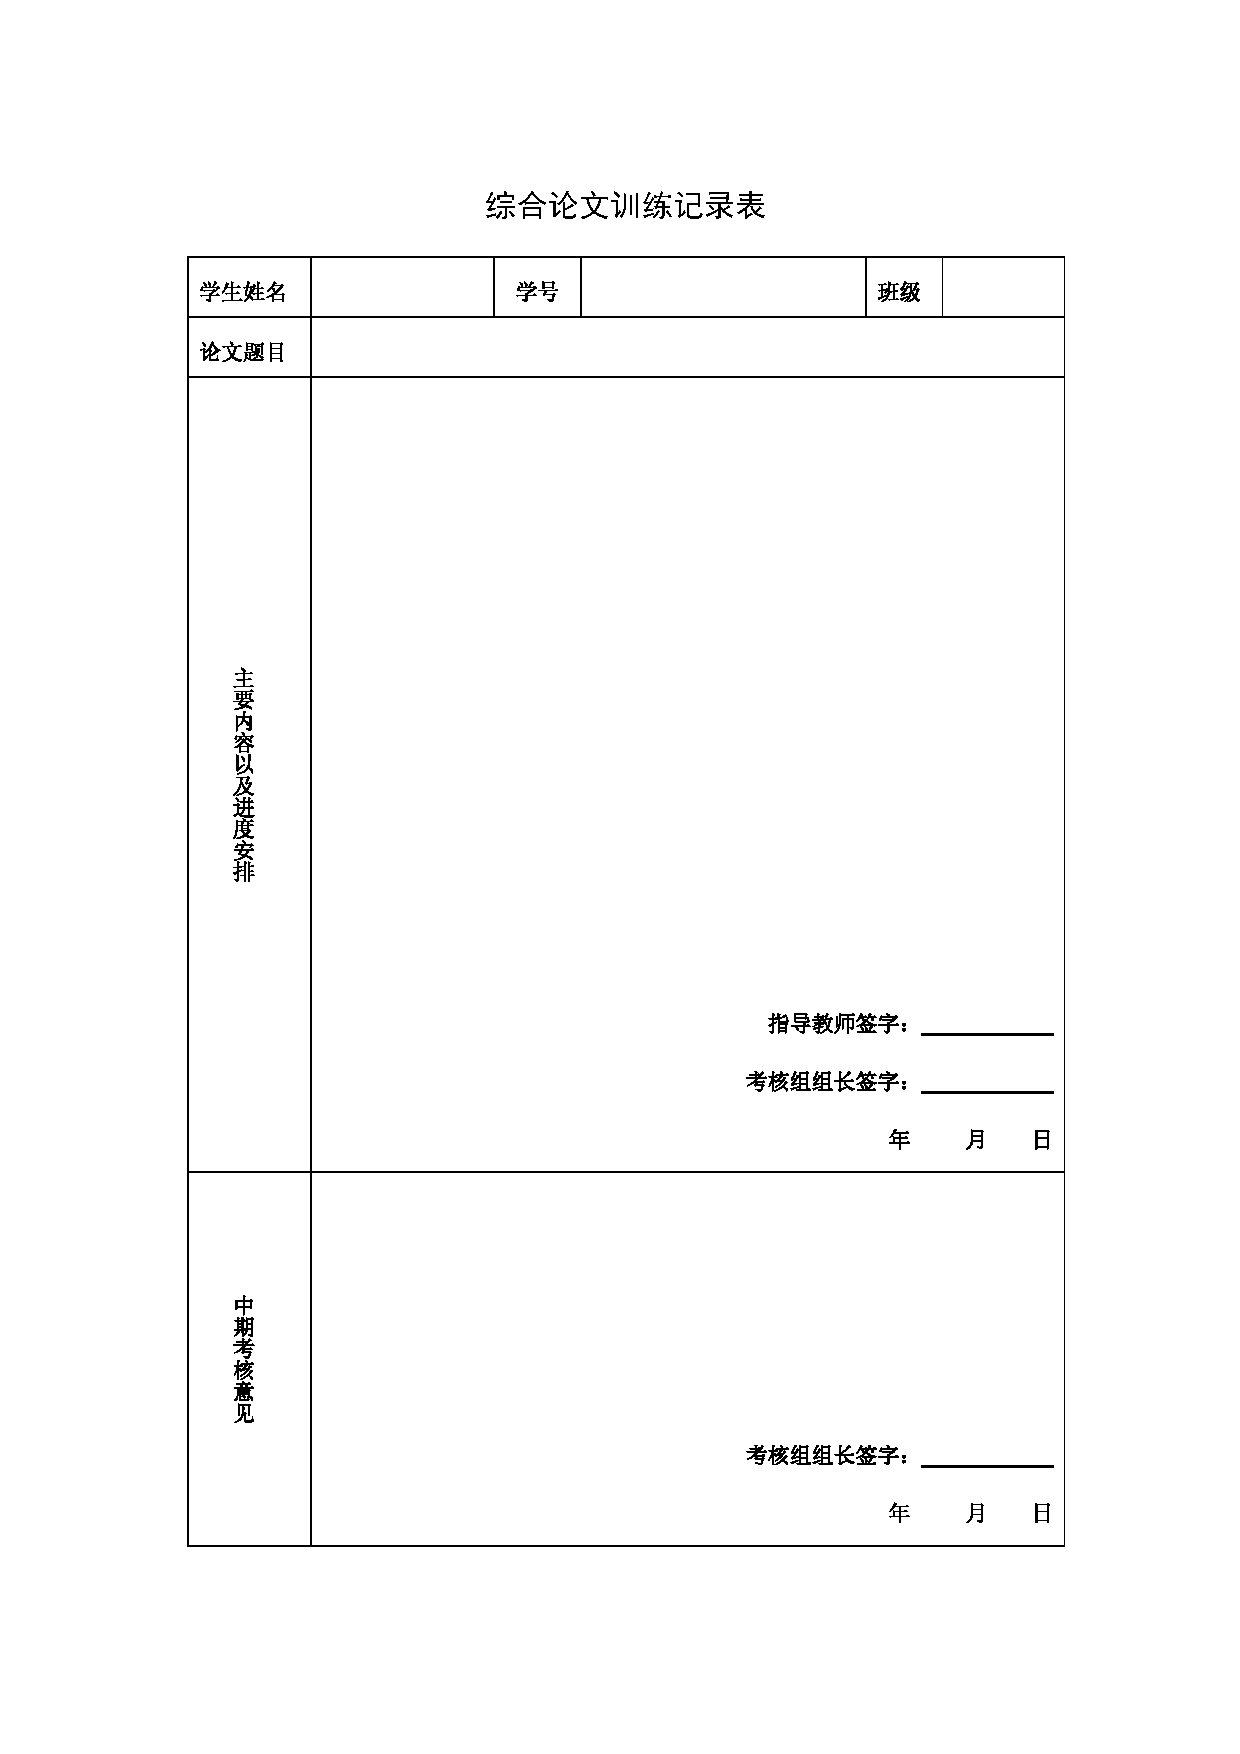
\includepdf[pages=-]{scan-record.pdf}
\end{document}
